\documentclass{article}

\usepackage[dutch]{babel}
\usepackage[margin=3cm]{geometry}
\usepackage{graphicx}
\usepackage{float}
\usepackage{caption}
\usepackage{hyperref}
\usepackage{amsmath}
\usepackage{wrapfig}
\usepackage[parfill]{parskip}

% fonts
\usepackage[T1]{fontenc}
\usepackage{helvet}
\renewcommand{\familydefault}{\sfdefault}

\graphicspath{{img/}}

% theorem environment
\usepackage{amssymb}

\newtheorem{theorem}{Definitie}[section]

\usepackage{enumitem}

\newenvironment{thmenum}
 {\begin{enumerate}[label=\upshape\bfseries(\roman*)]}
 {\end{enumerate}}


% code
\usepackage{minted}
\setminted{frame=single,framesep=3pt,linenos}
\usepackage{upquote}
\usepackage{color}

\begin{document}

\begin{titlepage}
    \author{Tuur Vanhoutte}
    \title{Advanced Programming \& Maths}
\end{titlepage}

\pagenumbering{gobble}
\maketitle
\newpage
\tableofcontents
\newpage

\pagenumbering{arabic}

\section{Basisfuncties in de wiskunde}

\subsection{Functies}

\begin{theorem}[Reële functie]
Een reële functie is een relatie in $\mathbb{R}$ waarbij elke waarde $x$ hoogstens één beeldwaarde $f(x)$ heeft
\end{theorem}

\begin{figure}[H]
    \centering
    \includegraphics[width=0.5\textwidth]{reele-functie.png}
    \caption{Voorbeelden reële functies}
\end{figure}

\begin{theorem}
Voor elke functie geldt: er bestaat een \dots
    \begin{thmenum}
        \item \dots domein van de functie (domain)
        \item \dots beeld van de functie (range)
        \item \dots functievoorschrift van de functie
    \end{thmenum}
\end{theorem}

\begin{figure}[H]
    \centering
    \includegraphics[width=0.5\textwidth]{functie-domain-range.png}
    \caption{Domein, bereik, functievoorschrift}
\end{figure}

$f: \mathbf{domein} \rightarrow \mathbf{bereik}: x \rightarrow y = f(x)$

$f: \mathbb{R} \rightarrow \mathbb{R} : x \rightarrow y = x^3 - 4x$

\begin{theorem}
    Elke functie kan nulpunten hebben.
\end{theorem}

\begin{figure}[H]
    \centering
    \includegraphics[width=0.5\textwidth]{functie-nulpunten.png}
    \caption{$y=-x^3 + 4x$}
\end{figure}

Verloop van een functie wordt via een tekenschema verduidelijkt:

\begin{figure}[H]
    \centering
    \includegraphics[width=0.5\textwidth]{functie-tekenschema.png}
    \caption{Tekenschema}
\end{figure}

\subsection{Veelterm en veeltermfuncties}

\begin{theorem}[Veelterm]
\begin{equation}
    \begin{aligned}
        A(x) &= a_nx^n + a_{n-1}x^{n-1} + a_{n-2}x^{n-2} + ... + a_{2}x^{2} + a_1x + a_0\\
        & (a_n,a_{n-1},...,a_2,a_1,a_0 \in \mathbb{R})
    \end{aligned}
\end{equation}

\end{theorem}

\begin{theorem}[Veeltermfunctie]
\begin{equation}
    \begin{aligned}
        f(x) &= a_nx^n + a_{n-1}x^{n-1} + a_{n-2}x^{n-2} + ... + a_{2}x^{2} + a_1x + a_0\\
        & Graad\ van\ veelterm\ = n\ (als\ a_n \neq 0)
    \end{aligned}
\end{equation}
\end{theorem}

\subsection{Bijzondere veeltermfuncties}

\begin{itemize}
    \item Constante functie: $f(x) = 4$
    \item Lineaire functie: $f(x) = 3x+6$
    \item Tweedegraadsfunctie: $f(x) = 3x^2 + 2x + 1$
    \item Derdegraadsfunctie: $f(x) = 5x^3 - 3x^2 + 2x - 1$
    \item Exponentiële functie: $f(x) = 2^x$
    \item Logaritmische functie: $(fx) = log_2(x)$
\end{itemize}

\subsubsection{Constante functie}

\begin{figure}[H]
    \centering
    \includegraphics[width=0.3\textwidth]{functie-constant.png}
    \caption{$y=4$}
\end{figure}

\subsubsection{Lineaire functie}

\begin{theorem}[Lineaire functie]
    \begin{equation}
        f(x) = ax + b
    \end{equation}


Voorbeeld: $f(x) = 3x + 6$
\end{theorem}

\begin{itemize}
    \item Betekenis van a: de richtingscoëfficiënt (rico)
    \item Betekenis van b: het snijpunt met de y-as
    \item Nulpunt: $f(x) = 0 \\ \Leftrightarrow 3x + 6 = 0 \\ \Leftrightarrow 3x = -6  \\ \Leftrightarrow x = -2$
\end{itemize}

\begin{figure}[H]
    \centering
    \includegraphics[width=0.3\textwidth]{functie-lineair2.png}
    \caption{Meerdere evenwijdige lineaire functies}
\end{figure}

Evenwijdige rechten als: als $a_1 = a_2$

Loodrechte rechten als: als $a_1 \cdot a_2 = -1$

\subsubsection{Tweedegraadsfunctie}

\begin{theorem}
\begin{equation}
    \begin{aligned}
        f(x) = ax^2 + bx + c,\\
        (a \neq 0)
    \end{aligned}
\end{equation}


\end{theorem}

\begin{figure}[H]
    \centering
    \includegraphics[width=0.2\textwidth]{functie-2degraad.png}
    \caption{$f(x) = x^2 - 2x - 3$}
\end{figure}

\begin{itemize}
    \item Betekenis van a: positief $\Rightarrow$ dalparabool, negatief $\Rightarrow$ bergparabool
    \item Nulpunten: via de discriminant berekenen:
\end{itemize}

\begin{theorem}[Discriminant]
Bij een tweedegraadsvergelijking is de discriminant:

\begin{equation}
    D = b^2 - 4ac
\end{equation}
\end{theorem}

\begin{itemize}
    \item Geval 1: $D > 0 \Rightarrow$ de functie heeft 2 nulpunten
    \item Geval 2: $D = 0 \Rightarrow$ de functie heeft 1 nulpunt
    \item Geval 3: $D < 0 \Rightarrow$ de functie heeft géén nulpunten
\end{itemize}

\begin{figure}[H]
    \centering
    \includegraphics[width=0.4\textwidth]{functie-2degraad3.png}
    \includegraphics[width=0.3\textwidth]{functie-2degraad2.png}
    \caption{De discriminant toont de nulpunten}
\end{figure}

\textbf{Nulpunten berekenen:} 

\begin{equation}
    x_{1,2} = \frac{-b \pm \sqrt{D}}{2a}
\end{equation}

\begin{figure}[H]
    \centering
    \includegraphics[width=0.5\textwidth]{functie-2degraad4.png}
    \caption{Symmetrieas: $x = \frac{-b}{2a}$}
\end{figure}

Hoe steil verloopt de grafiek? 

\begin{figure}[H]
    \centering
    \includegraphics[width=0.5\textwidth]{functie-2degraad5.png}
    \caption{$y = x^2 - 6x + 8$}
\end{figure}

\subsubsection{Derdegraadsfunctie}

\begin{theorem}[Derdegraadsfunctie]
\begin{equation}
    \begin{aligned}
        f(x) = ax^3 + bx^2 + cx + d
        (a \neq 0)
    \end{aligned}
\end{equation}


\end{theorem}

\subsubsection{Exponentiële functie}

\begin{theorem}[Exponentiële functie]
\begin{equation}
    f(x) = a^{g(x)}
\end{equation}

Met grondtal $a \in \mathbb{R}_0^+ \backslash \{1\}$
\end{theorem}

\begin{figure}[H]
    \centering
    \includegraphics[width=0.3\textwidth]{functie-exponentieel.png}
    \includegraphics[width=0.3\textwidth]{functie-exponentieel2.png}
\end{figure}


\begin{itemize}
    \item Betekenis van a: groeifactor
    \item Wanneer stijgend? 
    \item Wanneer dalend? 
    \item Nulpunten: 
    \item Vaststelling beeld functie
\end{itemize}



\begin{theorem}[Constante van Euler]

\begin{equation}
    \begin{aligned}
        e \approx 2.718281828\dots
    \end{aligned}
\end{equation}

$f(x) = e^x$ is een bijzondere exponentiële functie
\end{theorem}

\begin{figure}[H]
    \centering
    \includegraphics[width=0.5\textwidth]{functie-exponentieel3.png}
    \caption{Verschil tussen $2^x$, $3^x$ en $e^x$}
\end{figure}

\section{Exponentiële verbanden in data}

\subsection{Lineaire groei}

Kenmerkend:

\begin{itemize}
    \item Per tijdseenheid wordt hetzelfde getal \textbf{opgeteld}
    \item Grafiek is een rechte
    \item \textbf{Algemene formule} (N = aantal, t = tijd, b = beginhoeveelheid): 
    \begin{equation}
        N = a\cdot t + b
    \end{equation}
\end{itemize}

\begin{figure}[H]
    \centering
    \includegraphics[width=0.5\textwidth]{lineaire-groei.png}
    \caption{Lineaire groei}
\end{figure}

\subsection{Exponentiële groei}

Kenmerkend: 

\begin{itemize}
    \item Per tijdseenheid wordt de hoeveelheid met hetzelfde getal \textbf{vermenigvuldigd}
    \item Grafiek is een exponentiële functie
    \item \textbf{Algemene formule} (N = aantal, t = tijd, b = beginhoeveelheid, g = groeifactor): 
    \begin{equation}
        N = b \cdot g^t
    \end{equation}
\end{itemize}

\begin{figure}[H]
    \centering
    \includegraphics[width=0.5\textwidth]{exponentiele-groei.png}
    \caption{Exponentiële groei}
\end{figure}

\begin{figure}[H]
    \centering
    \includegraphics[width=0.5\textwidth]{voorbeeld-groei.png}
    \caption{Voorbeeld exponentiële groei met groeifactor $\approx 1.22$}
\end{figure}


\subsection{Van groeipercentage naar groeifactor}

De toename/afname wordt vaak ook procentueel uitgedrukt

\begin{itemize}
    \item Een jaarlijkse toename van $14.6\%$
    \item Een jaarlijkse afname van $14.6\%$
\end{itemize}

\begin{theorem}[Groeifactor]
De groeifactor is de factor die per tijdseenheid wordt vermenigvuldigd met de vorige waarde.
\end{theorem}

\subsubsection{Percentage naar factor}

\begin{equation}
g = \frac{p + 100}{100}\%
\end{equation} 

\begin{figure}[H]
    \centering
    \includegraphics[width=0.5\textwidth]{percentage-naar-factor.png}
    \caption{Van groeipercentage naar groeifactor}
\end{figure}


\subsubsection{Factor naar percentage}

\begin{figure}[H]
    \centering
    \includegraphics[width=0.35\textwidth]{factor-naar-percentage.png}
    \caption{Van groeifactor naar groeipercentage}
\end{figure}

\begin{figure}[H]
    \centering
    \includegraphics[width=0.5\textwidth]{groeifactoren.png}
    \caption{Let op: hier gebeuren vaak fouten bij het omrekenen}
\end{figure}

\subsection{Voorbeeld exponentiële groei}

Een hoeveelheid groeit exponentieel. Na 5u is $N = 82$ en na 12u is $N = 246$.

Stel de formule van N op.

\textbf{Oplossing}

\begin{equation*}
N = b \cdot g^t
\end{equation*}

\underline{Stap 1: groeifactor berekenen per tijdseenheid:}

\begin{center}
$$
\left.
    \begin{array}{lll}
        \text{Na 5u}  & \rightarrow & N = 82 \\
        \text{Na 12u} & \rightarrow & N = 246 \\
    \end{array}
\right \} \Delta = 7u \rightarrow 164
$$


Groeifactor voor 7 uren: $\frac{246}{82} = 3$

Groeifactor voor 1 uur: $3^{1/7} \approx 1.170$
\end{center}

\underline{Stap 2: 1 punt nemen waarvan we N weten:}

\begin{center}

Gekozen punt: $(5, 82)$

$82 = b \cdot (1.170)^5$

$\Leftrightarrow b = \frac{82}{1.170}^5 \approx 37$

$\Leftrightarrow N = 37 \cdot 1.170^t$
\end{center}

\subsection{Belangrijke maten voor exponentiële toename}


\begin{theorem}[Verdubbelingstijd]
De verdubbelingstijd is de nodige tijd tot de hoeveelheid verdubbeld is.

De verdubbelingstijd $t$ kan je berekenen door het omrekenen van deze formule:
\begin{equation}
g^t = 2
\end{equation}
\end{theorem}

\textbf{Oefening}

De populatie neemt toe met $8.3\%$ per jaar. Bereken de verdubbelingstijd:

\begin{center}
$g^t = 2$

$\Leftrightarrow (1.083)^t = 2$

$\Leftrightarrow \log(1.083^t) = \log(2)$

$\Leftrightarrow t \cdot \log(1.083) = \log(2)$

$\Leftrightarrow t = \frac{\log(2)}{\log(1.083)}$

$\Leftrightarrow t = 8.69\ jaar$

\end{center}


\begin{theorem}[Halveringstijd]
De halveringstijd is de nodige tijd tot de hoeveelheid gehalveerd is.

De halveringstijd $t$ kan je berekenen door het omrekenen van deze formule:
\begin{equation}
g^t = 1/2
\end{equation}
\end{theorem}

\subsubsection{Oefening: Combinatie van groeifactoren?}

Een hoeveelheid neemt eerst 5 jaar lang met vast percentage (*) toe, 
om daarna nog 3 jaar met 10\% per jaar toe te nemen. Na 8 jaar is
de totale hoeveelheid verdubbeld.

(*) Bereken het jaarlijkse groeipercentage in de eerste 5 jaren.

\textbf{Oplossing}

We weten:

\begin{itemize}
    \item Eerste 5 jaar: toename met vast percentage
    \item Volgende 3 jaar: toename met 10\% (= factor van 1.1)
    \item Na 8 jaar: hoeveelheid verdubbeld (= factor van 2)
\end{itemize}

\begin{align*}
g^5 \cdot 1.1^3 = 2
\end{align*}

We moeten $g$ vinden:

\begin{align*}
\Leftrightarrow g^5 = \frac{2}{1.1^3}\\
\Leftrightarrow g = \sqrt[5]{\frac{2}{1.1^3}}
\end{align*}

\section{Belangrijke functies met betrekking tot machine learning}

\subsection{Logistische groei}

\subsubsection{Voorbeeld}

Startsituatie: een bos (bv $\text{10km}^2$) waarin een konijnenepidemie uitbreekt.
Boswachter houdt de populatie van de konijnen bij. Wat stelt hij vast?

De groei van de populatie verloopt volgens een typisch patroon (niet exponentieel):

\begin{figure}[H]
    \centering
    \includegraphics[width=0.5\textwidth]{logistische-groei-vs-exponentieel.png}
    \caption{De rode lijn is de bovengrens}
\end{figure}

\subsubsection{De groei}

= de mate van toename

\begin{itemize}
    \item Hangt af van hoeveel er al zijn tegenover hoeveel er nog bij kunnen
    \item Heel sterke verandering bij start, op het einde heel kleine verandering
    \item Hangt dus ook af van de tijd
\end{itemize}

\begin{theorem}[De logistische groei]
De logistische groei is de mate van toename, afhankelijk van hoeveel er nog bij kan en hoeveel er al is

\begin{equation}
    \frac{\text{Hoeveel er nog bij kan}}{\text{Hoeveel er al is}} = B \cdot g^t
\end{equation}

\begin{itemize}
    \item $t =$ de tijd,
    \item $B$ en $g =$ constanten
\end{itemize}


\end{theorem}

\subsubsection{Functievoorschrift}

\begin{equation}
y = \frac{G}{1 + B\cdot g^t}
\end{equation}

\begin{itemize}
    \item $t =$ de tijd,
    \item $B$ en $g =$ constanten,
    \item $G =$ bovengrens
\end{itemize}

\begin{figure}[H]
    \centering
    \includegraphics[width=0.5\textwidth]{logistische-groei.png}
    \caption{Grafiek logistische groei met $G = 800$}
\end{figure}

\subsubsection{Voorbeeld}

Het aantal vissen in een meer is gegeven door:

\begin{center}
    $N = \frac{2500}{1 + 5.5 \cdot 0.74^t}$
\end{center}

waarbij $N =$ aantal vissen, $t =$ tijd

\textbf{Beredeneer}: Wanneer bereiken we het 'verzadigingsniveau'

Als t heel groot is:

\begin{itemize}
    \item Dan wordt $0.74^t \approx 0$
    \item Dan wordt $5.5 \cdot 0.74^t \approx 0$
    \item Dan wordt $N \approx 2500$
    \item $\Rightarrow$ Het meer is `verzadigd'
\end{itemize}

\subsubsection{Algemene wiskundige notatie van een logistische functie}

\begin{theorem}[Logistische functie]
De wiskundige notatie voor een logistische functie is:

\begin{equation}
    f(x) = \frac{c}{1 + a\cdot b^x}
\end{equation}

met $a,b,c$ constanten waarbij de constante $c$ de belangrijkste is:

c drukt uit wat de maximumwaarde kan zijn
\end{theorem}

\begin{figure}[H]
    \centering
    \includegraphics[width=0.5\textwidth]{logistische-functie-wiskundig.png}
\end{figure}

\subsection{Regression analysis}

Regressieanalyse:

\begin{itemize}
    \item Is er een (voorspellend) verband tussen 2 variabelen
    \item Heeft de ene variabele een invloed op de andere variabele
\end{itemize}

\begin{figure}[H]
    \centering
    \includegraphics[width=0.5\textwidth]{regressie.png}
    \caption{Regressieanalyse}
\end{figure}

\begin{figure}[H]
    \centering
    \includegraphics[width=0.5\textwidth]{regressie2.png}
    \caption{Lineaire vs niet-lineaire samenhang}
\end{figure}


\subsubsection{Lineair regressiemodel}

Enkelvoudige vorm: 

\begin{itemize}
    \item 1 inputwaarde $x$
    \item via lineaire functie $h_{\theta}(x) = \theta_0 + \theta_1x$
\end{itemize}

\begin{figure}[H]
    \centering
    \includegraphics[width=0.3\textwidth]{lineair-regressiemodel.png}
\end{figure}

\begin{itemize}
    \item Aan de hand van de opgestelde functie doe je een voorspelling
    \item \textbf{Doel:} een zo goed mogelijke lineaire functie opstellen
    \item $\Rightarrow$ zoektocht naar de beste $\theta_0$ en $\theta_1$
\end{itemize}


\subsubsection{Logistisch regressiemodel}

Logistische regressie = \textbf{Classificatie-algoritme}

Zoeken naar een model dat uitkomst (2 mogelijkheden) voorspelt mbv inputwaardes.
Elke inputwaarde heeft een zeker belang (gewicht).

\begin{figure}[H]
    \centering
    \includegraphics[width=0.5\textwidth]{regressiemodel.png}
    \caption{3 inputs met elk een bepaald gewicht, die een uitkomst zoekt (2 mogelijkheden)}
\end{figure}

Vereenvoudiging:  

\begin{itemize}
    \item 1 inputwaarde $x$
    \item Logistische functie $p = \frac{1}{1 + e^{-(b_0+b_1x)}}$
\end{itemize}

Uitkomst:

\begin{itemize}
    \item de persoon slaagt als $h_{\theta}(x) \geq 0.5$
    \item de persoon slaagt niet als $h_{\theta}(x) < 0.5$
\end{itemize}

\begin{figure}[H]
    \centering
    \includegraphics[width=0.3\textwidth]{logistisch-regressiemodel.png}
    \caption{1 inputwaarde $x$, met twee  uitkomsten}
\end{figure}

\subsubsection{Lineair vs logistisch regressiemodel}

\begin{figure}[H]
    \centering
    \includegraphics[width=0.5\textwidth]{lineair-vs-logistisch-regression-model.png}
    \caption{Hoe dichter p tegen 1, hoe zekerder het model is}
\end{figure}

Welk model gaat het snelst naar 0 en 1? 

\begin{itemize}
    \item Het logistische model
    \item Daarom is het logistische model beter voor classificatie: je splitst de groep op in 2
\end{itemize}

\subsubsection{Meerdere inputfactoren}

Zelfde redenering:

\begin{itemize}
    \item Meerdere inputwaardes $x_1, x_2, \dots$
    \item Gebruik $\theta_0 + \theta_1x_1 + \theta_2x_2 + \dots$
\end{itemize}

\begin{figure}[H]
    \centering
    \includegraphics[width=0.3\textwidth]{logistische-regressie-meerdere-inputfactoren.png}
    \caption{Regressiemodel met meerdere inputfactoren}
\end{figure}


\subsection{Softmax functie}

\begin{theorem}
    De softmax functie is een generalisatie van de logistische functie, die gebruikt kan worden om data
    te gaan categoriseren in verschillende klasses. Dat gebeurt met behulp van verschillende inputvariabelen en
    hun bijhorende parameters.
\end{theorem}

\begin{figure}[H]
    \centering
    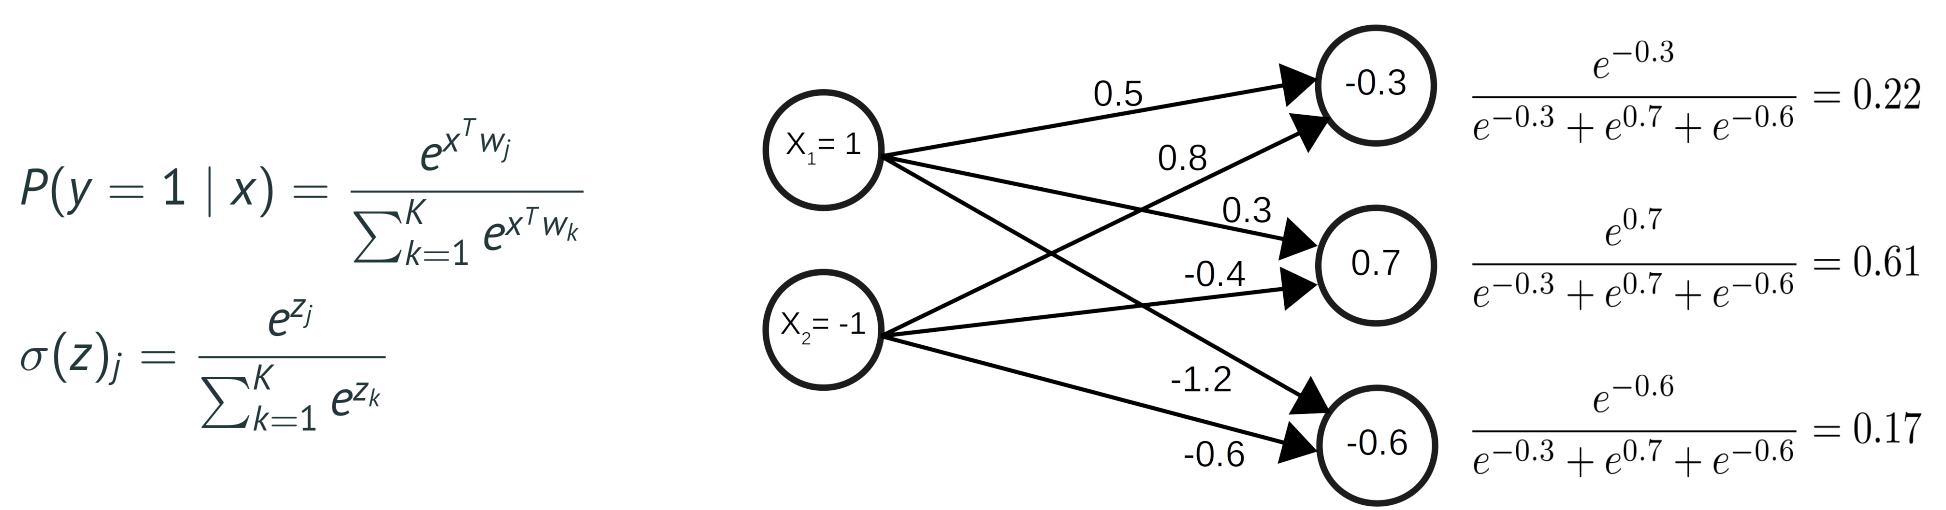
\includegraphics[width=0.35\textwidth]{softmax.png}
    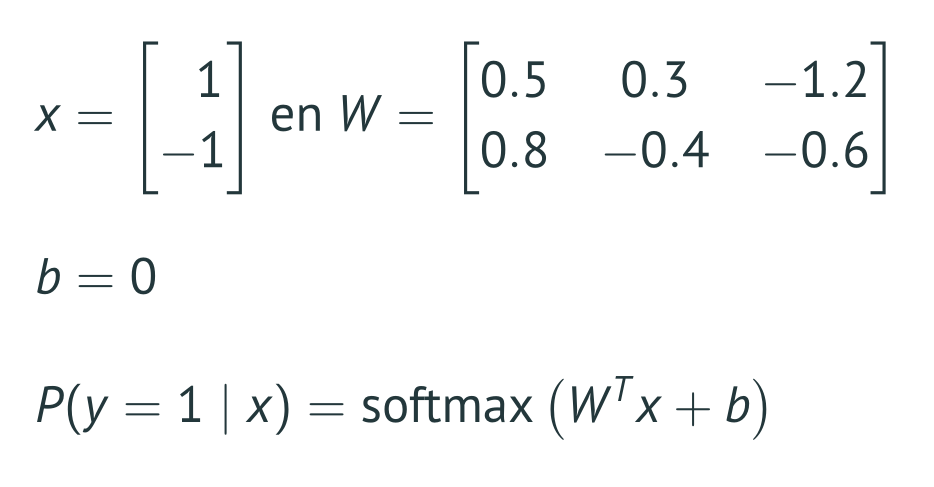
\includegraphics[width=0.4\textwidth]{softmax2.png}
    \caption{2 voorbeelden van categoriseren met de softmax functie}
\end{figure}

Let op: het is duidelijk dat softmax een probabiliteit zal geven aan elke klasse apart. 
De percentages tellen dus niet op tot 100\%.

\subsubsection{Kansen}

We berekenen de kansen dus per categorie. Met het bovenstaande voorbeeld van de dierherkenning: 
stel dat we 2 variabelen $x_1$ en $x_2$ hebben, met $x_1$ de grootte van de oren
en $x_2$ de grootte van de ogen. Dan kunnen we bijvoorbeeld stellen:

Kans dat de toestand tot groep $A$ behoort:

\begin{itemize}
    \item $\theta_{A,0} + \theta_{A,1}x_1 + \theta_{A,2}x_2$
    \item Voorbeeld: $0.01 + 0.1x_1 + 0.1x_2$
\end{itemize}

Kans dat de toestand tot groep $B$ behoort:

\begin{itemize}
    \item $\theta_{B,0} + \theta_{B,1}x_1 + \theta_{B,2}x_2$
    \item Voorbeeld: $0.1 + 0.2x_1 + 0.2x_2$
\end{itemize}

Kans dat de toestand tot groep $C$ behoort:

\begin{itemize}
    \item $\theta_{C,0} + \theta_{C,1}x_1 + \theta_{C,2}x_2$
    \item Voorbeeld: $0.1 + 0.3x_1 + 0.3x_2$
\end{itemize}

\subsubsection{Model}

Het softmax-model berekent de mate van zekerheid dat een toestand tot een bepaalde categorie behoort.

Volgende quotiënt drukt uit hoe zeker hij is dat $(x_1, x_2)$ tot categorie A behoort, met $(x_1, x_2)$ onze 2 variabelen:

\begin{align*}
    \frac{e^{\theta_{A,0} + \theta_{A,1}x_1 + \theta_{A,2}x_2}}{e^{\theta_{A,0} + \theta_{A,1}x_1 + \theta_{A,2}x_2} + e^{\theta_{B,0} + \theta_{B,1}z_1 + \theta_{B,2}z_2} + e^{\theta_{C,0} + \theta_{C,1}z_1 + \theta_{C,2}z_2} }
\end{align*}

(analoog voor categorie B en C: pas de teller aan)

\begin{figure}[H]
    \centering
    \includegraphics[width=0.9\textwidth]{softmax-voorbeeld.png}
    \caption{Betekenis: het model is 29\% zeker dat (0.1, 0.5) tot categorie A behoort. Bereken zelf als oefening voor B en C}
\end{figure}

\subsubsection{Wiskundig}

Het gebruikte model wordt via volgende wiskundige formule algemeen beschreven:

\begin{equation}
\frac{e^{x_k}}{\sum_{i=1}^n e^{x_i}}
\end{equation}

waarbij:

\begin{itemize}
    \item $x_k = \theta_{k,0} + \theta_{k,1}x_1 + \theta_{k,2}x_2 + \dots + \theta_{k,m}x_m$
    \item $n =$ aantal groepen
    \item $m =$ het aantal meetcriteria
\end{itemize}

\subsection{Logistic regression cost function}

Het model:

\begin{equation}
h_{\theta}(x) = \frac{1}{1 + e^{-\theta^{\tau}x}}
\end{equation}

waarbij:

\begin{itemize}
    \item $\theta^{\tau}x = \theta_0 + \theta_1x_1 + \theta_2x_2$
    \item $h_{\theta}$ drukt uit wat de kans is dat voor opgegeven $x_1$ en $x_2$ de waarneming tot 1 groep behoort
    \item $x_1$ en $x_2$ zijn de inputwaardes
    \item $\theta_1$ en $\theta_2$ zijn gewichten (hoe belangrijk is de input)
    \item \textbf{Doel: } vinden van de beste gewichten zodat de voorspelling == de werkelijkheid
\end{itemize}

\subsubsection{Succes meten}

\textbf{Stel:} je maakt een logistisch regressiemodel die bepaalt of een object een groene appel of een tennisbal is. 

\begin{itemize}
    \item Bepalen van de kostenfunctie $J(\theta)$ met als doel deze zo laag mogelijk te brengen
    \item Kost = afwijking tegenover de werkelijke situatie
    \item Werkelijkheid kan 2 situaties zijn:
    \begin{itemize}
        \item Indien de werkelijkheid een groene appel is $\Rightarrow y = 1$ 
        \item Indien de werkelijkheid géén groene appel is $\Rightarrow y = 0$ 
    \end{itemize}
\end{itemize}

Hoe ziet zo'n kostfunctie er dan uit?

\begin{figure}[H]
    \centering
    \includegraphics[width=0.4\textwidth]{logistische-regressie-kost.png}
    \caption{Als $y = 1$ en $y = 0$}
\end{figure}

\begin{figure}[H]
    \centering
    \includegraphics[width=0.3\textwidth]{logistische-regressie-kost2.png}
\end{figure}

\begin{figure}[H]
    \centering
    \includegraphics[width=0.4\textwidth]{logistische-regressie-kost3.png}
\end{figure}

Hoe brengen we 2 mogelijke situaties in 1 functie samen?

\begin{figure}[H]
    \centering
    \includegraphics[width=0.5\textwidth]{logistische-regressie-2situaties.png}
    \caption{Samenbrengen van de 2 situaties in 1 formule}
\end{figure}

\subsubsection{Kostenfunctie $J(\theta)$}

\begin{equation}
    J(\theta) = \frac{1}{m} \cdot \sum_{i=1}^m Cost(h_{\theta}(x_i), y_i)
\end{equation}

Kostenfunctie beschouwt alle gevallen:

\begin{itemize}
    \item Telkens kost berekenen
    \item Som berekenen van alle kosten om de gemiddelde kost te bepalen
\end{itemize}

\begin{figure}[H]
    \centering
    \includegraphics[width=0.5\textwidth]{logistische-regressie-kost-overzicht.png}
    \caption{Overzicht kostenfunctie}
\end{figure}

\subsubsection{Oefening}

Bereken zelf even de kost uit het voorbeeld uit de cursus Machine Learning. 
Het model is van de vorm: $h_{\theta}(x) = g(\theta_0 + \theta_1\cdot x_1 + \theta_2\cdot x_2)$

Met $x_1 =$ rondheid en $x_2 =$ groenheid.

Veronderstel na training: $\theta_0 = -40, \theta_1 = 4, \theta_2 = 4$

Met volgende waarnemingen: 

\begin{itemize}
    \item appel = meting rondheid 8, groenheid 6
    \item geen appel = meting rondheid 5, groenheid 4.5
\end{itemize}

\subsubsection{Extra}

Mooie blogpost: \url{https://adit.io/posts/2016-03-13-Logistic-Regression.html}


\section{Pandas library}

\subsection{Inleiding}

\begin{itemize}
    \item Doelstelling:
    \begin{itemize}
        \item Nut van de Pandas library kunnen situeren
        \item Data-analyse: basisbewerkingen
    \end{itemize}
    \item Pandas = `Python Data Analysis Library'
    \item Pandas bouwt op de NumPy library
    \item Officiële website: \url{https://pandas.pydata.org/}
    \item Goede start: \url{http://pandas.pydata.org/pandas-docs/stable/10min.html} 
\end{itemize}

\subsubsection{Welke data verwerken?}

\begin{itemize}
    \item csv-files
    \item txt-files
    \item Excel-files
    \item Databases
\end{itemize}

\subsection{Pandas.core}

Beschikbare datastructuren:

\begin{itemize}
    \item Series (1D)
    \item DataFrame (2D)
    \item Panel (3D)
\end{itemize}

\subsection{Series}

Bestemd voor 1-dimensionale data: 

`a one-dimension labeled array capable of holding any data'


\begin{itemize}
    \item Subklasse van numpy-ndarray
    \item Data: elk soort datatype
    \item Geordende index
    \item Duplicaten mag (maar niet optimaal)
\end{itemize}

\begin{figure}[H]
    \centering
    \includegraphics[width=0.2\textwidth]{panda-series.png}
    \caption{Elk element heeft een index}
\end{figure}

\subsection{DataFrame}

Bestemd voor meer-dimensionale data

\begin{itemize}
    \item Subklasse van numpy-ndarray
    \item Elke kolom kan ander datatype hebben
    \item Rij en kolom index
    \item Grootte wijzigbaar (invoegen/verwijderen van rijen en kolommen)
\end{itemize}

\begin{figure}[H]
    \centering
    \includegraphics[width=0.95\textwidth]{panda-dataframe0.png}
    \caption{DataFrames maken uit Python lists en dictionaries}
\end{figure}


\begin{figure}[H]
    \centering
    \includegraphics[width=0.25\textwidth]{panda-dataframe.png}
    \includegraphics[width=0.35\textwidth]{panda-dataframe2.png}
    \caption{Elk element heeft een rij en kolom}
\end{figure}


\subsubsection{Select data from DataFrame}

\textbf{Via operator [] selecteer je een kolom:}

\begin{figure}[H]
    \centering
    \includegraphics[width=0.3\textwidth]{panda-dataframe-data.png}
    \caption{Voorbeeld DataFrame}
\end{figure}


\begin{minted}{python}
# selecteer de kolom Jan uit dataframe
df['Jan']

# analoog: elke kolom is dus een attribuut van dataframe
df.Jan

# returnwaarde: Series-object
0   150
1   200
2   50
Name: Jan, dtype: int64
\end{minted}

\textbf{Via operator [[]] selecteer je een kolom \& krijg je een dataframe terug:}

\begin{minted}{python}
>> df[['Jan']]
# returns:
    Jan
0   150
1   200
2   50

>> df[['Jan', 'Mar']]
# returns:
    Jan     Mar
0   150     140
1   200     215
2   50      95
\end{minted}

\textbf{Via de operator [] en met een conditie:}

\begin{figure}[H]
    \centering
    \includegraphics[width=0.3\textwidth]{panda-dataframe-data2.png}
    \caption{Voorbeeld DataFrame}
\end{figure}

\begin{minted}{python}
>> df[df.Jan > 60]
# returns:
    Feb     Jan     Mar     account
0   200     150     140     Jones LLC
1   210     200     215     Alpha Co

>> df[np.logical_and(df.Jan > 100, df.Feb <= 200)]
# returns:
    Feb     Jan     Mar     account
0   200     150     140     Jones LLC

>> df[df.account.str.startswith(‘Alpha’)]
# test deze eens zelf uit als oefening :)
\end{minted}

\subsubsection{Veelgebruikte commando's bij dataframes}

\begin{minted}{python}
df.shape            # geeft de dimensie als een tuple terug
df.info()           # oplijsting van de aanwezige kolommen
df.head([aantal])   # eerste vijf/aantal rijen
df.tail([aantal])   # laatste vijf/aantal rijen
df.index            # geef de index-kolom weer
df.colums           # geef de kolomnamen weer
df.describe()       # geef snel overzicht van statistische data
df.T                # transponeer data (rij -> kol, kol -> rij)
df.sort_index()     # sorteer op basis van index
df.sort_values()    # sorteren op één of meerdere kolommen
\end{minted}


\subsection{Loc vs iloc}

\subsubsection{iloc}

= Integer-location based indexing / selection by position

\begin{itemize}
    \item Nut: selecteren van rijen en kolommen via rij/kolomnummer
    \item Syntax: data.iloc[<row>, <column>]
    \item Returnwaarde:
    \begin{itemize}
        \item Indien 1 \textbf{rij} $\Rightarrow$ series-object
        \item Indien meerdere \textbf{rijen}: $\Rightarrow$ dataframe-object
        \item 1 of meerdere \textbf{kolommen}: $\Rightarrow$ dataframe-object 
    \end{itemize}
\end{itemize}

\textbf{iloc-voorbeelden:}

\begin{minted}{python}
# Rows:
data.iloc[0] # first row of data frame
data.iloc[1] # second row of data frame
data.iloc[-1] # last row of data frame

# Columns:
data.iloc[:,0] # first column of data frame
data.iloc[:,1] # second column of data frame
data.iloc[:,-1] # last column of data frame

data.iloc[0:5] # first five rows of dataframe

# first two columns of data frame with all rows
data.iloc[:, 0:2] 

# 1st, 4th, 7th, 25th row + 1st 6th 7th columns.
data.iloc[[0,3,6,24], [0,5,6]]  

# first 5 rows and 5th, 6th, 7th columns of data frame
data.iloc[0:5, 5:8]

\end{minted}

\subsubsection{loc}

= lable-based indexing / selection

\begin{itemize}
    \item Nut: selecteren van rijen en kolommen via label / via conditionele look-up
    \item Syntax: data.loc[<row>, <column>]
    \item Returnwaarde:
    \begin{itemize}
        \item Indien 1 \textbf{rij/kol} $\Rightarrow$ series-object
        \item Indien meerdere \textbf{rijen}: $\Rightarrow$ dataframe-object
        \item 1 of meerdere \textbf{kolommen}: $\Rightarrow$ dataframe-object 
    \end{itemize}
\end{itemize}


\textbf{loc-voorbeelden:}

\begin{figure}[H]
    \centering
    \includegraphics[width=0.4\textwidth]{pandas-loc-voorbeeld.png}
    \caption{Voorbeeld dataframe}
\end{figure}


\begin{minted}{python}
reviews.loc[:2, "score"] # return type = 

reviews.loc[:2, ["score", "title"]] # return type = 

# select column "score" where value of index <= 5
reviews.loc[:5, "score"]

# select columns "country" and "cars_per_cap" where rowindex is "US" or "RU"
cars.loc[ ["US","RU"] , ["country","cars_per_cap"]]

# select columns "country" and "cars_per_cap" where rowindex is from "US" to "RU"
cars.loc[ "US " : "RU " , ["country","cars_per_cap"]]

# selectie rijen hoeft niet altijd op basis van row-index te zijn
# select columns "country" and "drives_right", voor de landen 'Japan' en 'India'
cars.loc[ cars.country.isin( ['Japan', 'India'] ) , ['country','drives_right']]
\end{minted}

\subsection{Plotten met pandas}

\subsubsection{Dataframe plotten}

\begin{minted}{python}
# print(cars[['country', 'cars_per_cap']])
# werkwijze 1:
cars[['country', 'cars_per_cap']].plot(kind='bar', legend=True)
# werkwijze 2:
cars.plot(x='country', y='cars_per_cap', kind='bar', legend=True)

plt.show()
\end{minted}

\begin{figure}[H]
    \centering
    \includegraphics[width=0.4\textwidth]{pandas-plotting.png}
    \caption{Resultaat}
\end{figure}

\subsubsection{Series plotten}

\begin{minted}{python}
# werkwijze 1:
plt.plot(cars['cars_per_cap'])
# werkwijze 2:
plt.plot(cars['cars_per_cap'].plot(color='r', legend=True))

plt.show()
\end{minted}

\begin{figure}[H]
    \centering
    \includegraphics[width=0.4\textwidth]{pandas-plotting2.png}
    \caption{Resultaat}
\end{figure}

\subsection{Demo: Iris Dataset}

(Zie DemoPandas.zip op Leho voor de code)

\begin{figure}[H]
    \centering
    \includegraphics[width=0.5\textwidth]{pandas-demo.png}
    \caption{Een iris bestaat uit petals \& sepals, met elk hun breedte en lengte}
\end{figure}

\begin{figure}[H]
    \centering
    \includegraphics[width=0.5\textwidth]{pandas-demo2.png}
    \caption{Plotten van de beschikbare data (demo5.py)}
\end{figure}

\begin{figure}[H]
    \centering
    \includegraphics[width=0.3\textwidth]{pandas-demo3.png}
    \caption{Vergelijken van de lengtes en breedtes adhv box-plots (demo6.py)}
\end{figure}

\begin{minted}{python}
# filteren van data
result_check = iris['Species'] == 'Iris-setosa'
# print(type(result_check)) == <class 'pandas.core.series.Series'>
filtered_setosa = iris.loc[result_check, :]
# of in 1 lijn:
filtered_setosa = iris.loc[iris['Species'] == 'Iris-setosa', :]
\end{minted}

\begin{figure}[H]
    \centering
    \includegraphics[width=0.3\textwidth]{pandas-demo4.png}
    \includegraphics[width=0.4\textwidth]{pandas-demo5.png}
    \caption{Frequentiediagram voor de Iris-setosa soort (demo7.py)}
\end{figure}

\subsection{Complexe bewerkingen}

\begin{figure}[H]
    \centering
    \includegraphics[width=0.8\textwidth]{pandas-complexe-bewerkingen.png}
    \caption{Reshaping data: change the layout of a data set}
\end{figure}

\section{Normaaldistributie}

\subsection{Doelstellling}

\begin{itemize}
    \item Het herkennen van van de eigenschappen van de normaalverdeling
    \item Verband standaard normaalverdeling en Z-waarden
    \item Z-index, Z-score tabel
\end{itemize}

\subsection{Inleiding}

Wanneer komt een normaalverdeling voor?

\begin{itemize}
    \item Grote aantallen onafhankelijke waarnemingen uit een willekeurige populatie
    \begin{itemize}
        \item De lengte van personen
        \item Productieprocessen die een bepaalde tijdsduur hebben
        \item \dots
    \end{itemize}
\end{itemize}

\subsection{Basisbegrippen}

\begin{theorem}[Normaalverdeling]
    Een intervalwaarde dat afhankelijk is van oneindig aantal onafhankelijke factoren (die los van elkaar in werken)
    zal in de populatie een normaalverdeling vertonen (Gauss-curve)

    \begin{figure}[H]
        \centering
        \includegraphics[width=0.3\textwidth]{gauss.png}
        \caption{Gauss-curve}
    \end{figure}
\end{theorem}

\subsubsection{Kenmerken}

\begin{itemize}
    \item Klokvormig verloop
    \item 1 maximum = gemiddelde = mediaan ($\mu$)
    \item Uitslagen vooral geconcentreerd rond gemiddelde
    \item Frequentie daalt naarmate scores afwijken
    \item Twee buigpunten: ($\mu - \sigma$ en $\mu + \sigma$)
    \item Symmetrie
\end{itemize}

\begin{figure}[H]
    \centering
    \includegraphics[width=0.4\textwidth]{gauss-kenmerken.png}
    \caption{Kenmerken Gauss-curve}
\end{figure}

\begin{itemize}
    \item Standaarddeviatie (standaardafwijking) $\sigma$ weerspiegelt mate van spreiding
    \item Wordt gemeten in de buigpunten
\end{itemize}

\begin{figure}[H]
    \centering
    \includegraphics[width=0.4\textwidth]{gauss-buigpunt.png}
\end{figure}

\begin{itemize}
    \item Functie is volledig te beschrijven met het gemiddelde $\mu$ en de Standaarddeviatie $\sigma$
\end{itemize}

\begin{figure}[H]
    \centering
    \includegraphics[width=0.4\textwidth]{gauss-notatiewijze.png}
    \caption{Notatiewijze}
\end{figure}

\begin{figure}[H]
    \centering
    \includegraphics[width=0.6\textwidth]{gauss-verschillend.png}
    \caption{Impact $\mu$ en $\sigma$}
\end{figure}

\subsubsection{Verdeling}

\begin{figure}[H]
    \centering
    \includegraphics[width=0.4\textwidth]{gauss-verdeling.png}
\end{figure}

\begin{figure}[H]
    \centering
    \includegraphics[width=0.4\textwidth]{gauss-verdeling2.png}
\end{figure}


\begin{itemize}
    \item Tussen beide buigpunten ($\mu - \sigma$, $\mu + \sigma$): $\approx68\%$ van de populatie
    \item Tussen ($\mu - 2\cdot\sigma$, $\mu + 2\cdot\sigma$): $\approx95\%$ van de populatie
    \item Tussen ($\mu - 3\cdot\sigma$, $\mu + 3\cdot\sigma$): $\approx99\%$ van de populatie
\end{itemize}

\subsubsection{Gevolg: Kansberekening}

\begin{itemize}
    \item Oppervlakte onder de grafiek = 100\%
    \item Hiermee kunnen we nu uitdrukken wat de kans van een specifiek bereik kan zijn. Bv:
    \begin{itemize}
        \item Met $\mu = 78, \sigma = 9 \Rightarrow $ Kans dat $x < 65$? 
        \item $\Rightarrow$ bereken oppervlakte links van 65
    \end{itemize}
\end{itemize}

\subsubsection{Wiskundig}

\begin{equation}
f(x) = \frac{1}{\sqrt{2\cdot\pi}\cdot \sigma}\cdot e^{-\frac{(x - \mu)^2}{2\cdot\sigma^2}}
\end{equation}

Standaardafwijking berekenen:

\begin{equation}
    \sigma = \sqrt{\frac{\sum_{i=1}^n (x_i - \mu)^2}{n - 1}}
\end{equation}

\begin{itemize}
    \item $\sigma =$ Standaarddeviatie van getallenreeks $x$
    \item $x_i =$ de waarde van getal $i$ in de getallenreeks
    \item $\mu =$ het gemiddelde van de getallenreeks
    \item $n =$ het aantal getallen in de proef
\end{itemize}

\subsection{Standaard normaalverdeling}

\begin{theorem}[Standaard normaalverdeling]
    De standaardnormaalverdeling is een normaalverdeling waarbij:
    
    \begin{itemize}
        \item $\mu = 0$
        \item $\sigma = 1$
    \end{itemize}
\end{theorem}


\begin{figure}[H]
    \centering
    \includegraphics[width=0.4\textwidth]{standaardnormaalverdeling.png}
    \caption{Oppervlakte onder grafiek $=1$}
\end{figure}

\subsubsection{Standaardiseren van een normaalverdeling}

\begin{theorem}
    Een normaalverdeling omzetten in een standaardnormaalverdeling waarbij $\mu = 0$ en $\sigma = 1$ noemen we het standaardiseren van die normaalverdeling.
\end{theorem}


\begin{figure}[H]
    \centering
    \includegraphics[width=0.4\textwidth]{standardizeren.png}
    \caption{Standaardiseren}
\end{figure}

\begin{itemize}
    \item Willekeurige normaalverdeling: $X \sim N(\mu, \sigma^2)$
    \item Verschuiven naar $0$: $X - \mu$
    \item samendrukken/uitrekken tot $\sigma = 1$: $\frac{X - \mu}{\sigma}$
\end{itemize}


\begin{figure}[H]
    \centering
    \includegraphics[width=0.4\textwidth]{gestandardizeerd.png}
    \caption{Gestandaardiseerd: alle eigenschappen blijven bewaard, enkel de hoogte blijft hetzelfde}
\end{figure}


\begin{figure}[H]
    \centering
    \includegraphics[width=0.5\textwidth]{standardizering-voorbeeld.png}
    \caption{Standaardiseren: voorbeeld}
\end{figure}

\subsection{Kansberekening}

\begin{figure}[H]
    \centering
    \includegraphics[width=0.5\textwidth]{normaalverdeling-kansen.png}
    \caption{$Z \sim N(0, 1) \rightarrow \mu = 0$ en standaardafwijking $\sigma = 1$}
\end{figure}

\begin{itemize}
    \item Grafiek beschrijft hoe waarschijnlijk uitkomsten zijn
    \item Uitkomsten dicht bij 0 waarschijnlijker dan in de staarten
    \item Kans = oppervlakte onder de grafiek, totale kans = 100\% = 1
\end{itemize}

\subsubsection{Via tabellen}

\begin{figure}[H]
    \centering
    \includegraphics[width=0.4\textwidth]{normaalverdeling-tabel.png}
    \includegraphics[width=0.3\textwidth]{normaalverdeling-tabel2.png}
    \caption{Kansberekening via tabellen: rijen = 1 getal na de komma, kolommen = 2de getal na de komma. $P(Z < 1.25) = 0.1056$}
\end{figure}

\begin{itemize}
    \item Symmetrie: $P(Z < -1.25) = P(Z > 1.25) = 0.1056$
    \item Complement: $P(Z < -1.25) = 1- P(Z < 1.25)$
\end{itemize}

\subsection{Z-score}

\begin{theorem}[Z-score]
    Een Z-score geeft aan hoeveel standaardafwijkingen een observatie van het gemiddelde verwijderd is.

    Je krijgt dus je plek ten opzichte van het gemiddelde, uitgedrukt in een
    standaard maat.

    \textbf{Voordeel:} je weet direct hoe goed iemand scoort ten opzichte van de
    rest.
\end{theorem}

\subsubsection{Wiskundig}

\begin{equation}
    z = \frac{x - \mu}{\sigma}
\end{equation}

\subsubsection{Voorbeeld}

\begin{figure}[H]
    \centering
    \includegraphics[width=0.5\textwidth]{z-score.png}
    \caption{Hoeveel standaarddeviaties ($\sigma$) zit een score van het gemiddelde $\mu$}
\end{figure}

\textbf{Voorbeeld:} 20 studenten leggen een examen af.

\begin{itemize}
    \item Gemiddelde $\mu = 7/10$
    \item Standaardafwijking $\sigma = 0.5$ ($68\%$ heeft score tussen $[6.5, 7.5]$)
    \item Iemand heeft $6/10 \Rightarrow$ z-score $= -2 \Rightarrow 2\cdot 0.5$ onder gemiddelde 
\end{itemize}

\subsubsection{Nut}

Z-score is eveneens een uitdrukking van de kans:

\begin{itemize}
    \item Hoe (on)gebruikelijk is een score
    \item Bij vorig voorbeeld: $2.275\%$ heeft een score $\leq 6/10$
\end{itemize}

\begin{figure}[H]
    \centering
    \includegraphics[width=0.25\textwidth]{z-score-nut.png}
\end{figure}

\subsection{Scheefheid}

Veel frequentieverdelingen hebben niet de vorm van de normaalverdeling. Ze zijn `scheef'

\begin{figure}[H]
    \centering
    \includegraphics[width=0.5\textwidth]{scheefheid.png}
    \caption{Scheefheid}
\end{figure}

\begin{itemize}
    \item Linksscheef = gemiddelde is lager dan de mediaan
    \item Rechtscheef = gemiddelde is hoger dan de mediaan
\end{itemize}

\begin{figure}[H]
    \centering
    \includegraphics[width=0.3\textwidth]{scheefheid2.png}
\end{figure}

\subsubsection{Berekening}

De maat voor scheefheid kan berekend worden:

\begin{itemize}
    \item Linksscheef: negatieve waarde
    \item Rechtsscheef: positieve waarde
\end{itemize}

\begin{equation}
    Scheefheid = \Bigg(\frac{(\frac{\sum(x - \bar{x})^3}{n})}{(\frac{\sum(x - \bar{x})^2}{n})^{3/2}}\Bigg)
\end{equation}

Interpretatie:

\begin{itemize}
    \item Waarde tussen [-0.5, 0.5]: zeer goede normaalverdeling
    \item Waarde tussen [-1, 1]: redelijk goede normaalverdeling
    \item Waarde daarbuiten: geen goede normaalverdeling
\end{itemize}

\subsection{Kurtosis}

\begin{theorem}[Kurtosis]
    Kurtosis is de maat van de gepiektheid. 

    Je gaat na of de verdeling een scherpe top heeft of een nogal vlakke top.
\end{theorem}

\begin{figure}[H]
    \centering
    \includegraphics[width=0.5\textwidth]{kurtosis.png}
\end{figure}

\subsubsection{Wiskundig}

\begin{equation}
    Kurtosis = \Bigg(\frac{\frac{\sum(x-\bar{x})^4}{n}}{(\frac{\sum(x-\bar{x})^2}{n})^2} \Bigg) -3
\end{equation}

Interpretatie:

\begin{itemize}
    \item $0$ = normaalverdeling
    \item Minimum is $-3$: volledig plat
    \item Maximum is $+\inf$
\end{itemize}


\subsection{Anomaly detection}

Voorbeeld: suikerfabriek produceert 1kg suikerzakken

\begin{itemize}
    \item In werkelijkheid: nooit exact 1kg
\end{itemize}

\begin{figure}[H]
    \centering
    \includegraphics[width=0.8\textwidth]{anomaly-detection.png}
    \caption{Verdeling 1kg suikerzak}
\end{figure}

\begin{theorem}[Anomalie]
    Een anomalie in een normaalverdeling is een onregelmatigheid of afwijking

    Soms verdacht, soms niet

    "Anomaly detection (also outlier detection) is the identification of items,
    events or observations which do not conform to an expected pattern or
    other items in a dataset."
\end{theorem}

\subsubsection{Detectiemethode 1}

= Minimum- en maximumgrens vastleggen

Bv:

\begin{itemize}
    \item wanneer een waarde kleiner is dan $\mu - 4\sigma$ (920 gram)
    \item wanneer een waarde groter is dan $\mu + 4\sigma$ (1080 gram)
\end{itemize}

\begin{figure}[H]
    \centering
    \includegraphics[width=0.4\textwidth]{anomaly-detection2.png}
\end{figure}

\subsubsection{Detectiemethode 2}

= detecteren van een zeldzame verdeling die afwijkt van de normaalverdeling

Bv:

\begin{itemize}
    \item 4 opeenvolgende waarden die vallen in de buitengrenzen $\mu - 3\sigma$ en $\mu + 3\sigma$
    \item Kans voor 1 waarde: $0.3\%$
    \item Kans voor 4 opeenvolgende waardes: $(0.3\%)^4 = (0.003)^4 = 0.000000000081$
    \item Het is duidelijk dat 4 opeenvolgende waardes heel zelden voorkomen $\Rightarrow$ anomalie
\end{itemize}

Bv: 

\begin{itemize}
    \item 50 opeenvolgende waarden die vallen in de buitengrenzen $\mu - \sigma$ en $\mu + \sigma$
    \item Kans voor 1 waarde: $68\%$
    \item Kans 50 opeenvolgende waardes: $(0.68)^{50} = 4.221 \cdot 10^{-9}$
    \item Heel lage kans $\Rightarrow$ anomalie
\end{itemize}

\begin{figure}[H]
    \centering
    \includegraphics[width=0.4\textwidth]{anomaly-detection3.png}
\end{figure}


\subsubsection{Detectiemethode 3}

De tweede techniek kan dus een vreemde afwijking van de normaalverdeling detecteren, maar
het kan geen anomalieën detecteren die van de ene sigma naar de andere gaan op een normale manier.

Om deze soort anomalie te detecteren moeten we kijken naar een `window' van de laatste $n$ elementen.
Als het gemiddelde en de standaardafwijking te veel variëren in die window, kunnen we vaststellen dat er een anomalie is.


\begin{figure}[H]
    \centering
    \includegraphics[width=0.4\textwidth]{anomaly-detection4.png}
    \caption{Oplossing: gebruik van window}
\end{figure}

\section{Kansrekening}

Doelstelling: 

\begin{itemize}
    \item Basiskennis kansrekening
    \item Definitie van Laplace
    \item Somregel kunnen toepassen
    \item Wet van de grote getallen
    \item Wat is een empirische kans?
\end{itemize}

\subsection{Basiskennis}

Kansrekenen = waarschijnlijkheidsrekenen

\begin{itemize}
    \item Vrij jonge tak in de wiskunde
    \item `Rekenen over wat er nog niet is'
\end{itemize}

\subsubsection{Voorbeeld}

Wat is de kans dat je 6 ogen gooit met een dobbelsteen?

\begin{itemize}
    \item Kans op gooien van 1 = 1/6
    \item Kans op gooien van 2 = 1/6
    \item \dots
    \item Kans op gooien van x = 1/6 = 16.7\%
\end{itemize}

1 = aantal gunstige uitkomsten

6 = aantal mogelijke uitkomsten

\subsection{Kansdefinitie van Laplace}

\begin{theorem}[Kansdefinitie van Laplace]
Bij een kansexperiment is de kans op een gebeurtenis $G$ gelijk aan:

$P(G) = \frac{\text{aantal gunstige uitkomsten}}{\text{aantal mogelijke uitkomsten}}$

\end{theorem}

\subsubsection{Wiskundige notatie}

\begin{equation}
    P(A) = \frac{\#A}{\#\Omega}
\end{equation}
    
\begin{itemize}
    \item Met $A$: een gebeurtenis
    \item Met $\Omega$: alle mogelijkheden (`het universum') ($\Omega = \{w_1, w_2, \dots, w_n\}$)
    \item Met $\#A$: aantal elementen (uitkomsten) die voldoen aan deze gebeurtenis
    \item Met $\#\Omega$: aantal elementen uit universum
    \item Voorwaarde: alle mogelijke uitkomsten zijn even waarschijnlijk
\end{itemize}

\subsubsection{Gecombineerd experiment}

\textbf{Bv: je gooit 2 dobbelstenen}

Wat is de kans op de gebeurtenis `de som is 6 ogen'?

\begin{itemize}
    \item $P(\text{som} == 2) = \frac{1}{36}$
    \item $P(\text{som} == 6) = \frac{5}{36}$
\end{itemize}

\begin{figure}[H]
    \centering
    \includegraphics[width=0.5\textwidth]{gecombineerd-experiment.png}
    \caption{Kans dat de som 6 ogen is}
\end{figure}

Wat is de kans op de gebeurtenis `de som is minstens 9 ogen'?

\begin{itemize}
    \item $P(\text{som} >= 9) = \frac{10}{36} = \frac{5}{18}$
\end{itemize}

\begin{figure}[H]
    \centering
    \includegraphics[width=0.5\textwidth]{gecombineerd-experiment2.png}
    \caption{Kans dat de som minstens 9 ogen is}
\end{figure}

\textbf{Oefening}: je gooit met een gewone dobbelsteen en een viervlaksdobbelsteen

\begin{itemize}
    \item Wat is de kans op de gebeurtenis met beide dobbelstenen evenveel gooien?
    \begin{itemize}
        \begin{figure}[H]
            \centering
            \includegraphics[width=0.4\textwidth]{gecombineerd-experiment-oef1.png}
            \caption{Kansentabel opstellen}
        \end{figure}
        \item $P(\text{beide dobbelstenen evenveel}) = \frac{4}{24} = \frac{1}{6}$
    \end{itemize}
    \item Wat is de kans dat de som van de ogen minstens 8 is?
    \begin{itemize}
        \item Opnieuw kansentabel opstellen $\Rightarrow \frac{6}{24} = \frac{1}{4}$ 
    \end{itemize}
\end{itemize}

\subsection{Somregel}

Bv: Je gooit met 2 dobbelstenen

\begin{itemize}
    \item Wat is de kans op `som is 3 \textcolor{red}{of} som is 5'
    \begin{figure}[H]
        \centering
        \includegraphics[width=0.4\textwidth]{somregel.png}
        \caption{Geen overlap: }
    \end{figure}
    
    \item Wat is de kans op `verschil is 1 \textcolor{red}{of} product is 12'
    \begin{figure}[H]
        \centering
        \includegraphics[width=0.4\textwidth]{somregel2.png}
        \caption{Er is overlap: gevaar voor dubbeltelling $\Rightarrow$ verschil aftrekken}
    \end{figure}
\end{itemize}

\subsubsection{Wiskundig}

\begin{itemize}
    \item De gebeurtenis dat A of B beide optreden = $A \cup B$ `vereniging'
    \item De gebeurtenis dat A of B tegelijkertijd optreden = $A \cap B$ `doorsnede'
\end{itemize}

\begin{theorem}[Somregel]
De kans dat de vereniging zich voordoet `som-regel':

\begin{equation}
    P(A \cup B) = P(A) + P(B) - P(A \cap B)
\end{equation}

Als $P(A \cap B)$ leeg is, dan geldt:

\begin{equation}
    P(A \cup B) = P(A) + P(B)
\end{equation}
\end{theorem}

\subsubsection{Algemene somregel}

Voor 3 gebeurtenissen A,B,C

\begin{equation}
    \begin{aligned}
        P(A \cup B \cup C) &= P(A) + P(B) + P(C)\\
        & - P(A \cap B) - P(A \cap C) - P(B \cap C)\\
        & + P(A \cap B \cap C)
    \end{aligned}
\end{equation}



\begin{figure}[H]
    \centering
    \includegraphics[width=0.4\textwidth]{algemene-somregel.png}
    \caption{$A \cap B \cap C$ moet terug opgeteld worden want hij werd te veel afgetrokken}
\end{figure}

\subsection{Complementregel}

1 dobbelsteen:

\begin{itemize}
    \item Je gooit een 6
    \item Verzameling van alle andere mogelijke gebeurtenissen = complement van die gebeurtenis
    \item Complement van een 6 gooien == alles behalve een 6 gooien
\end{itemize}

\begin{theorem}
    De complementregel stelt dat een gebeurtenis $G$ en zijn complement $G_{\text{complement}}$ samen alle mogelijkheden vormen.

    \begin{equation}
        \begin{aligned}
            P(G) + P(G_{\text{complement}}) = 1\\
            \Leftrightarrow P(G) = 1 - P(G_{\text{complement}})
        \end{aligned}
    \end{equation}
\end{theorem}

\subsection{Samengesteld of stochastisch experiment}

\begin{theorem}
    Een stochastisch kansexperiment is een experiment dat een aantal keer herhaald wordt.
\end{theorem}

Verschillende oplossingsmethodes mogelijk:

\begin{itemize}
    \item Kansboom
    \item Combinaties
\end{itemize}

\textbf{Voorbeeld}: in een vaas liggen 5 briefjes waarop telkens 1 letter staat: 3 briefjes met de letter A en twee briefjes met de letter B

2 mogelijkheden: 

\begin{itemize}
    \item trekking met teruglegging
    \item trekking zonder teruglegging
\end{itemize}

\subsubsection{Trekking met teruglegging}

Uit de vaas wordt lukraak een letter getrokken. Deze wordt genoteerd
en teruggelegd. Vervolgens trekken we opnieuw een letter.

\begin{figure}[H]
    \centering
    \includegraphics[width=0.5\textwidth]{trekking-met-teruglegging-kansboom.png}
    \caption{Verloop voorgesteld via een kansboom}
\end{figure}

\begin{itemize}
    \item Uitkomstenverzameling: $U = \{AA, AB, BA, BB\}$
    \item Elke tak = bijhorende deelkans
\end{itemize}

\begin{theorem}[Onafhankelijke deelexperimenten]
    Kansen bij de tweede trekking zijn onafhankelijk van het resultaat van de eerste trekking
\end{theorem}

Wat is $P(AB)$?

\begin{itemize}
    \item N = groot aantal herhalingen
    \item $\frac{3}{5}N$ keer leveren een A op
    \item $\frac{2}{5}N$ keer leveren een B op
    \item \textbf{Gevolg:} $\frac35 \frac25 N$ keer volgen de weg AB
    \item $\Rightarrow$ $P(AB) = \frac{6}{25}$
\end{itemize}

\begin{figure}[H]
    \centering
    \includegraphics[width=0.4\textwidth]{trekking-met-teruglegging-tabel.png}
\end{figure}


\textbf{Productregel voor kansen:} De kans op een weg is gelijk aan het product van de kansen langs die weg
    

\subsubsection{Trekking zonder teruglegging}

Uit de vaas wordt lukraak een letter genomen. Deze wordt genoteerd en \textcolor{red}{niet} teruggelegd.
Vervolgens trekken we een nieuwe letter

\begin{figure}[H]
    \centering
    \includegraphics[width=0.3\textwidth]{trekking-zonder-teruglegging-kansboom.png}
    \includegraphics[width=0.4\textwidth]{trekking-zonder-teruglegging-tabel.png}
    \caption{We vermenigvuldigen opnieuw de kansen}
\end{figure}


\begin{theorem}[Afhankelijke deelexperimenten]
    Kansen bij de tweede trekking zijn afhankelijk van het resultaat van de eerste trekking
\end{theorem}

\subsection{Permutaties}

\begin{theorem}[Permutatie]
    Een permutatie van een verzameling elementen is een herschikking of herordening ervan.

    $\Rightarrow$ volgorde is van belang! 
\end{theorem}

\subsubsection{Voorbeeld:} 

Je organiseert een wedstrijd voor 10 hardlopers. 

Op hoeveel manieren kan ik de gouden/zilveren/bronzen medaille gaan verdelen?

\begin{itemize}
    \item Volgorde van belang!
    \item Aantal permutaties van 3 uit 10: $10 \cdot 9 \cdot 8 = 720$
\end{itemize}

\subsubsection{Oefeningen}

Een reclameblok bestaat uit 9 items: 2 over eten, 3 over reizen, 4 over auto's

\begin{enumerate}
    \item Op hoeveel manieren kunnen deze items gerangschikt worden?
    \begin{itemize}
        \item $9 \cdot 8 \cdot 7 \cdot 6 \cdot 5 \cdot 4 \cdot 3 \cdot 2 \cdot 1 = 9! = 362880$
    \end{itemize}
    \item Op hoeveel manieren kunnen deze items gerangschikt worden als de items over reizen direct na elkaar komen?
    \begin{itemize}
        \item Aantal manieren om reizen te rangschikken: $3!$
        \item Aantal manieren om de rest te rangschikken: $7!$
        \item Eindoplossing: $3! \cdot 7!$
    \end{itemize}
\end{enumerate}

\subsection{Combinaties}

\begin{theorem}[Combinaties]
    Een combinatie is een aantal manieren om $k$ dingen uit $n$ dingen te kiezen \textbf{zonder} dat de volgorde van belang is.
\end{theorem}

\subsubsection{Wiskundig}

`n boven k' of `uit n kies ik er k'

\begin{equation}
    \binom{n}{k} = \frac{n!}{(n-k)! \cdot k!}
\end{equation}

\subsubsection{Voorbeeld}

Uit 63 studenten worden er 8 gekozen om deel te nemen aan de studentenparticipatie

$\binom{63}{8} = \frac{63!}{(63-8)! \cdot 8!} = 3 872 894 697$


\subsubsection{Oefening}

We gooien met 5 identieke muntstukken. Wat is de kans dat we 3 \textbf{of} 4 keer kop gooien?

\begin{itemize}
    \item Gevraagd: $P(3\ \text{keer kop of}\ 4\ \text{keer kop})$
    \item Totaal = $2 \cdot 2 \cdot 2 \cdot 2 \cdot 2 = 2^5 = 32$
    \item Aantal gunstige:
    \begin{itemize}
        \item 3x kop: $\binom{5}{3} = 10$
        \item 4x kop: $\binom{5}{4} = 5$
    \end{itemize}
    \item Resultaat: somregel = $P(3\ \text{keer kop of}\ 4\ \text{keer kop}) = \frac{10}{32} + \frac{5}{32} = \frac{15}{32}$
\end{itemize}

\subsection{Theoretische en empirische kansen}

\subsubsection{Theoretische kansen:}

\begin{itemize}
    \item Eenvoudige kansberekeningen: gooien van een dobbelsteen, kans dat je 5 gooit
    \item Dit is een `theoretische' of `a priori' kans:
    \begin{itemize}
        \item De kans op een gebeurtenis is vooraf berekenbaar
    \end{itemize}
\end{itemize}

\subsubsection{Empirische kansen}

\begin{itemize}
    \item Complexere kansberekening
    \item Uitkomst niet eenvoudig berekenbaar
\end{itemize}


\subsubsection{Voorbeeld}
We gooien 60 keer met een dobbelsteen, hoeveel vijven verwacht je hierbij?

\begin{itemize}
    \item Verwachting: 10x1, 10x2, 10x3, \dots
    \item Maar is de werkelijkheid = verwachting?
    \item Relatieve frequentie: $\frac{\text{frequentie}}{\text{aantal worpen}} = \frac{10}{60} = \frac16$
\end{itemize}

\begin{theorem}[De wet van de grote getallen]
    Wanneer we een experiment heel vaak herhalen komt de relatieve frequentie steeds dichter in de buurt van de kans op de gebeurtenis.
\end{theorem}

\begin{figure}[H]
    \centering
    \includegraphics[width=0.5\textwidth]{wet-grote-getallen.png}
    \caption{De wet van grote getallen}
\end{figure}

\begin{itemize}
    \item Nuttig wanneer we kans niet vooraf kunnen berekenen.
    \item Door het experiment heel vaak te herhalen, kunnen we de kans afleiden.
    \item Hierdoor mogelijkheid tot uitspraak over experiment in toekomst
    \item Dit heet \textbf{de empirische kans}: de kans gebaseerd op waarneming
\end{itemize}

\subsubsection{Voorbeeld 2}

Experiment met duimspijker: op hoeveel manieren kan hij bij een worp op de grond komen?

\begin{itemize}
    \item We bekijken de kans P(punt omlaag) en P(punt omhoog)
    \item Is dat wel 50/50?
    \item Theoretische kans niet te bepalen\dots
    \item Door experiment uit te voeren: de empirische kans $P(\text{punt omhoog}) \approx 0.58$
\end{itemize}

\section{Voorwaardelijke kans}

\subsection{Doelstelling}

\begin{itemize}
    \item Voorwaardelijke kansen berekenen
    \item Onafhankelijke gebeurtenissen herkennen
    \item Regel van Bayes kennen en  toepassen
\end{itemize}

\subsection{Situering}

Een patiënt heeft mogelijk last van griep, verkoudheid, of beide.

\begin{itemize}
    \item Een verkouden patiënt heeft met 60\% kans last van hoestbuien, met 10\% kans op hoofdpijnklachten
    \item Een patiënt met griep heeft kans 20\% op hoestbuien, met 70\% kans op hoofdpijn
\end{itemize}

Vragen

\begin{enumerate}
    \item De patiënt vertelt dat hij last heeft van hoestbuien. Hoe groot is de kans dat hij griep heeft?
    \item Hij zegt dat hij ook last heeft van hoofdpijn. Hoe groot is de kans nu dat hij griep heeft?
\end{enumerate}

\subsection{Voorbeeld}

Voorwaardelijke kans: kans die aan een voorwaarde voldoet

\begin{figure}[H]
    \centering
    \includegraphics[width=0.5\textwidth]{voorwaardelijke-kans-sport.png}
\end{figure}

Bereken exact de kans dat een willekeurig gekozen\dots

\begin{enumerate}
    \item \dots leerling 1 sport beoefend?
    \begin{itemize}
        \item P(leerling sport niet) = 39/71
    \end{itemize}
    \item \dots leerling een jongen is en niet sport?
    \begin{itemize}
        \item P(jongen 1 sport) = 5/71
    \end{itemize}
    \item \dots meisje meer dan 1 sport beoefend
    \begin{itemize}
        \item P(meisje >1 sport) = 7/\textcolor{red}{32}
    \end{itemize}
    \item \dots niet-sportende leerling een jongen is?
    \begin{itemize}
        \item P(niet sportende leerling is jongen) = 5/\textcolor{red}{13}
    \end{itemize}
    \item \dots meisje aan sport beoefend?
    \begin{itemize}
        \item P(meisje doet sport) = $\frac{17 + 7}{32} = \frac34$
    \end{itemize}
\end{enumerate}

Bij voorwaardelijke kansen bekijk je slechts een deel van de groep.
Het aantal mogelijke uitkomsten waar je door deelt is dus een deelgroep

\subsection{Wiskundig}

De kans dat B onder de voorwaarde van A gebeurt:
\begin{equation}
    P(B | A) = \frac{P(A \cap B)}{P(A)} = \frac{P(AB)}{P(A)}
\end{equation}

Indien alle elementen in A en B evenwaardig zijn:

\begin{equation}
    P(B | A) = \frac{P(A \cap B)}{P(A)} = \frac{\#(A \cap B)}{\#(A)}
\end{equation}

\subsubsection{Gevolg: productregel}

We weten:

$P(B|A) = \frac{P(AB)}{P(A)}$

$P(A|B) = \frac{P(AB)}{P(B)}$

Daaruit volgt:

\begin{equation}
    \begin{aligned}
        P(A \cap B) &= P(AB)\\
        &= P (B|A) \cdot P(A)\\
        &= P (A|B) \cdot P(B)
    \end{aligned}
\end{equation}

De kans dat A en B samen voorkomen:

\begin{itemize}
    \item = (kans op B onder voorwaarde van A) * kans op A
    \item = (kans op A onder voorwaarde van B) * kans op B
\end{itemize}

\subsubsection{Algemene productregel}

Met 3 verzamelingen:

\begin{equation}
    \begin{split}
        P(A \cap B \cap C) & = P(ABC)\\
        & = P(C | AB) \cdot P(AB)\\
        & = P(C | AB) \cdot P (B|A) \cdot P(A) 
    \end{split}
\end{equation}

\textbf{Algemeen:}

\begin{equation}
    P(ABC\dots Z) = P(Z|ABC\dots Y) \cdot \dots \cdot P (C| A B ) \cdot P(B|A) \cdot P(A)
\end{equation}

\subsection{Oefening 1}

\subsubsection{Opgave}

\begin{figure}[H]
    \centering
    \includegraphics[width=0.4\textwidth]{voorwaardelijke-kans-oef1.png}
    \caption{Opgave}
\end{figure}

\subsubsection{Oplossing}

Je vermenigvuldigt voor elke machine het productiepercentage met het defect percentage voor die machine. 
Die kansen tel je op:

\begin{center}
    \begin{align*}
        & P(D | M_1) \cdot P(M_1) + P(D | M_2) \cdot P(M_2) + P(D | M_3) \cdot P(M_3)\\
        & = 0.01 \cdot 0.2 + 0.02 \cdot 0.3 + 0.03 \cdot 0.5 \\
        & = 0.023
    \end{align*}
\end{center}

\subsection{Oefening 2}

\subsubsection{Opgave}

\begin{figure}[H]
    \centering
    \includegraphics[width=0.4\textwidth]{voorwaardelijke-kans-oef2.png}
    \caption{Opgave}
\end{figure}

\subsubsection{Oplossing}

\begin{center}
    \begin{align*}
        P(M_2 | D) & = \frac{P(M_2 \cap D)}{P(D)}\\
        & = \frac{P(D | M_2) \cdot P(M_2)}{P(D)}\\
        & = \frac{0.02 \cdot 0.3}{0.023}\\
        & = 0.261
    \end{align*}
\end{center}

\subsection{Onafhankelijke gebeurtenissen}

\subsubsection{Voorbeeld}

In een groep van 65 jongeren is er onderzoek gedaan of ze wel of niet sporten

3 gebeurtenissen:

\begin{itemize}
    \item A: een leerling sport
    \item B: een leerling is een jongen
    \item C: een leerling is een meisje
\end{itemize}

\begin{figure}[H]
    \centering
    \includegraphics[width=0.4\textwidth]{voorwaardelijke-kans-sport2.png}
\end{figure}

\begin{itemize}
    \item Kans dat een leerling sport: $P(A) = \frac{55}{65} = \frac{11}{13}$
    \item Kans dat een leerling sport onder voorwaarde dat het een jongen is: $P(A | B) = \frac{11}{13}$
    \item \textbf{Vaststelling:} of een leerling sport beoefend is onafhankelijk of het een jongen is
\end{itemize}

Wanneer gebeurtenis A en B onafhankelijk zijn geldt P(A onder voorwaarde B) = P(A)

\begin{itemize}
    \item Kans dat leerling een jongen is: $P(B) = \frac{13}{65}= \frac15$
    \item Kans dat leerling een jongen is onder de voorwaarde dat hij sport: $P(B|A) = \frac{11}{55}= \frac15$
\end{itemize}

Wanneer gebeurtenis A en B onafhankelijk zijn geldt P(A onder voorwaarde B) = P(A) en dus ook P(B voorwaarde A) = P(B)

\subsubsection{Gevolg: Productregel voor onafhankelijke gebeurtenissen}

Indien A en B onafhankelijk zijn, dan is de kans dat B onder voorwaarde van A gebeurt:

\begin{itemize}
    \item $P(B | A) = P(B)$
    \item $P(A | B) = P(A)$
\end{itemize}

Productregel wordt dan: 

\begin{equation}
    P(A \cap B) = P(B) \cdot P(A) = P(A) \cdot P(B)
\end{equation}

\subsection{Productregel algemeen}

Voor een n-tal willekeurige gebeurtenissen $A_1, A_2, \dots, A_n$ geldt:

\begin{equation}
    P(A_1 \cap A_2 \cap \dots \cap A_n) = P(A_1) \cdot P(A_2 | A_1) \dots P(A_n | A_1 \cap A_2 \cap \dots \cap A_{n-1})
\end{equation}

Men schrijft dit kort als:

\begin{equation}
    P(A_1 A_2 \dots A_n) = P(A_1) \cdot P(A_2 | A_1) \dots P(A_n | A_1 A_2 \dots A_{n-1})
\end{equation}

\subsubsection{Oefening 1}

Controleer of het hebben van blauwe ogen al dan niet afhankelijk is van het geslacht

\begin{figure}[H]
    \centering
    \includegraphics[width=0.5\textwidth]{vkans-productregel-oef.png}
    \caption{Opgave}
\end{figure}


\subsubsection{Oefening 2}

Controleer of kans op bloedgroep AB al dan niet onafhankelijk is van de waarde Rh+

\begin{figure}[H]
    \centering
    \includegraphics[width=0.5\textwidth]{vkans-productregel-oef2.png}
    \caption{Opgave}
\end{figure}

\subsection{Regel van Bayes}

\subsubsection{Toepassingsdomein}

\begin{itemize}
    \item Belangrijkste deel uit kansrekening
    \item Toepassing in medische en genetische diagnostiek, AI, organisatie van dataverkeer, wetenschappelijk onderzoek
\end{itemize}

\begin{figure}[H]
    \centering
    \includegraphics[width=0.5\textwidth]{bayes-voorbeeld1.png}
    \caption{Voorbeeld 1}
\end{figure}

\begin{figure}[H]
    \centering
    \includegraphics[width=0.5\textwidth]{bayes-voorbeeld2.png}
    \caption{Voorbeeld 2}
\end{figure}

\subsubsection{Formule van Bayes (eenvoudige vorm)}

Uit:

\begin{center}
    $P(A | B) = \frac{P(A \cap B)}{P(B)}$ en $P(B | A) = \frac{P(A \cap B)}{P(A)}$
\end{center}

volgt:

\begin{center}
    $P(A \cap B) = P(A | B) \cdot P(B) = P(B | A) \cdot P(A)$
\end{center}

dus:

\begin{equation}
    P(A | B) = \frac{P(A \cap B)}{P(B)} = \frac{P(B | A) \cdot P(A)}{P(B)}
\end{equation}

\subsubsection{Voorbeeld}

De kans dat een zekere kerncentrale oververhit raakt (O) is $1\cdot 10^{-7}$,
de kans dat een lek (L) ontstaat is $1\cdot 10^{-8}$, maar als er eenmaal
een lek is, is de kans groot dat de centrale oververhit raakt: $0.1$

Wat is de kans dat de centrale gaat lekken als hij oververhit raakt?

$P(L|O) = \frac{P(L\cap O)}{P(O)} = \frac{P(O|L)\cdot P(L)}{P(0=O)}$

Dus:

$P(L|O) = \frac{0.1 \cdot 1 \cdot 10^{-8}}{1\cdot 10^{-7}} = 0.01$


\subsection{Regel van Bayes (variant 1)}

We beschouwen van een gebeurtenis $H$ ook zijn complement $\bar{H}$.

Ter herinnering:

\begin{itemize}
    \item $P(B) + P(\bar{B}) = 1$
    \item $P(B|A) = \frac{P(B \cap A)}{P(A)}$
    \item $P(B|\bar{A}) = \frac{P(B \cap \bar{A})}{P(\bar{A})}$
\end{itemize}

Daaruit volgt:

\begin{equation*}
    \begin{aligned}
        P(B) & = P(B \cap A) + P(B \cap \bar{A})\\
        & = P(B | A) \cdot P(A) + P(B | \bar{A}) \cdot P(\bar{A})
    \end{aligned}
\end{equation*}

Dus als we \textcolor{red}{$P(B)$} integreren in de formule van Bayes:

\begin{equation}
    \begin{aligned}
        P(A|B) &= \frac{P(B|A) \cdot P(A)}{\textcolor{red}{P(B)}}\\
        &= \frac{P(B|A) \cdot P(A)}{\textcolor{red}{P(B|A)\cdot P(A) + P(B|\bar{A})\cdot P(\bar{A})}}
    \end{aligned}
\end{equation}

\begin{figure}[H]
    \centering
    \includegraphics[width=0.5\textwidth]{bayes-variant-voorbeeld1.png}
    \includegraphics[width=0.6\textwidth]{bayes-variant-voorbeeld1-opl.png}
    \caption{Voorbeeld 1}
\end{figure}

\begin{figure}[H]
    \centering
    \includegraphics[width=0.5\textwidth]{bayes-variant-voorbeeld2.png}
    \includegraphics[width=0.6\textwidth]{bayes-variant-voorbeeld2-opl.png}
    \caption{Voorbeeld 2}
\end{figure}

\subsection{Regel van Bayes (variant 2)}

We beschouwen van een gebeurtenis $H$ ook zijn complement $\bar{H}$, 
waarbij nu geldt dat $P(H) = P(\bar{H})$. We kunnen dus bepaalde termen schrappen:


\begin{equation}
    \begin{aligned}
        P(H | E) & = \frac{P(E | H) \textcolor{red}{\cdot P(H)}}{P(E | H) \textcolor{red}{\cdot P(H)} + P(E | \bar{H}) \textcolor{red}{\cdot P(\bar{H})}}\\
        & = \frac{P(E | H)}{P(E | H) + P(E | \bar{H})}
    \end{aligned}
\end{equation}

\subsection{Regel van Bayes (algemeen)}

Verzameling B in verschillende gevallen onderverdeeld $(B_1, B_2, \dots, B_n)$ die elkaar
uitsluiten: $B_i \cap B_j = \phi$ als $i \neq j$

\begin{equation}
    P(B_j | A) = \frac{P(A | B_j) \cdot P(B_j)}{\sum_{i=1}^n P(A|B_i) \cdot P(B_i)}
\end{equation}

\begin{figure}[H]
    \centering
    \includegraphics[width=0.5\textwidth]{bayes-algemeen-voorbeeld1.png}
    \includegraphics[width=0.6\textwidth]{bayes-algemeen-voorbeeld1-opl.png}
    \caption{Voorbeeld algemene regel van Bayes}
\end{figure}

\subsection{Bayesiaans leren: toepassing in machine learning}

\begin{theorem}
    Bayesiaans leren heeft in essentie de volgende vorm: Er zijn een aantal hypotheses $H_1, \dots, H_n$ die samen de uitkomstenverzameling vormen.

    De hypotheses zijn meer of minder waarschijnlijk: de (initiële) bijbehorende verdeling is de \textbf{a-priori verdeling}, de kansen
    $P(H_i)$ zijn de \textbf{a-priori kansen}
\end{theorem}

Na het verkrijgen van nieuwe informatie/data/gebeurtenis $E$ worden de kansen van de hypotheses aangepast volgens de stelling van Bayes:

\begin{equation}
    P(H_i | E) = \frac{P(E | H_i) \cdot P(H)}{\sum_{j=1}^n P(E | H_j) \cdot P(H_j)}
\end{equation}


\begin{itemize}
    \item De kansen $P(H_i | E)$ zijn de \textit{a-posteriori} kansen. 
    \item De kansen $P(E | H_i)$ zijn de \textit{likelihoods} van $E$
\end{itemize}

\subsubsection{Leren}

Op grond van telkens nieuwe data $E_1, E_2, \dots$ wordt de verdeling van de hypotheses voortdurend aangepast: $P_0, P_1, P_2, \dots$

\begin{itemize}
    \item $P_0$ is de a-priori verdeling, waarbij $P_0(H_i) = P(H_i)$
    \item Na het verkrijgen van data $E_1$ wordt de nieuwe verdeling $P_1$, waarbij $P_1(H_i) = P_0(H_i | E_1)$
    \item Na het verkrijgen van data $E_2$ wordt de nieuwe verdeling $P_2$, waarbij $P_2(H_i) = P_1(H_i | E_2)$
    \item \dots
\end{itemize}


\begin{figure}[H]
    \centering
    \includegraphics[width=0.5\textwidth]{bayesiaans-leren.png}
    \caption{Bayesiaans leren}
\end{figure}


\subsection{Naïve Bayes Spam Filter}

\textbf{Doelstelling:} Regel van Bayes kennen en toepassen om een eenvoudige spam-filter te programmeren.

\begin{itemize}
    \item Gegeven een bepaalde spamfilter
    \item Email komt in spamfolder: hoe groot is de kans dat het effectief spam is?
    \begin{itemize}
        \item $P(\text{spam} | \text{message}) = \frac{P(\text{message}|\text{spam}) \cdot P(\text{spam})}{P(\text{message})}$
        \item Waarbij: $P(\text{spam} | \text{message})=$ de kans dat een email uit spamfolder effectief spam is
        \item En: $P(\text{message}|\text{spam})=$ de kans op classificatie spam door deze filter
    \end{itemize}
    \item Email komt in inbox: hoe groot is de kans dat het geen spam is?
    \begin{itemize}
        \item $P(\neg \text{spam} | \text{message}) = \frac{P(\text{message}|\neg \text{spam}) \cdot P(\neg \text{spam})}{P(\text{message})}$
        \item Waarbij: $P(\neg \text{spam} | \text{message})=$ de kans dat een email uit inbox effectief geen spam is
        \item En: $P(\text{message}| \neg \text{spam})=$ de kans op classificatie geen spam door deze filter
    \end{itemize}
\end{itemize}

\begin{figure}[H]
    \centering
    \includegraphics[width=0.75\textwidth]{bayes-spam.png}
    \caption{Als links $>$ rechts $\Rightarrow$ email naar spamfolder, anders email naar inbox}
\end{figure}

Een gegeven e-mail (message) wordt dus herkend als spam als:

\begin{itemize}
    \item $P(\text{spam} | \text{message}) > P(\neg \text{spam} | \text{message})$
    \item Merk op dat $P(\text{message})$ geen invloed heeft op de beslissing
    \item Dus: $P(\text{message}|\text{spam}) \cdot P(\text{spam}) > P(\text{message}|\neg \text{spam}) \cdot P(\neg \text{spam})$
\end{itemize}

\subsubsection{Herkennen van een spam bericht}

Doel:

\begin{itemize}
    \item Berekenen van P(message|spam) P(spam)
    \item Berekenen van P(message|not spam) P(not spam)
\end{itemize}

Message:

\begin{itemize}
    \item opeenvolging van woorden ($w_1, w_2, \dots, w_n$)
    \item volgorde niet belangrijk
    \item elk woord is onafhankelijk van het andere woord
\end{itemize}

Berekenen van $P(\text{message}|\text{spam}) P(\text{spam})$:

\begin{align*}
    P(message|spam) & = P(w_1, w_2, \dots, w_n | \text{spam})\\
    & = P(w_1 | \text{spam}) \cdot P(w_1 | \text{spam}) \cdot \dots \cdot P(w_n | \text{spam})\\
    & = \prod_{i=1}^n P(w_i | \text{spam})
\end{align*}

Berekenen van $P(\text{message}|\neg \text{spam}) P(\neg \text{spam})$:

\begin{align*}
    P(message|spam) & = P(w_1, w_2, \dots, w_n |\neg \text{spam})\\
    & = \prod_{i=1}^n P(w_i | \neg \text{spam})
\end{align*}

Onze filter classificeert een message als spam als:

\begin{figure}[H]
    \centering
    \includegraphics[width=0.5\textwidth]{bayes-spam2.png}
\end{figure}

\subsubsection{Parameters}

\begin{itemize}
    \item $P(\text{spam})$
    \item $P(\neg \text{spam})$
    \item $P(\text{woord}|\text{spam})$
    \begin{itemize}
        \item = woord aantal keer gevonden in spam messages, gedeeld door aantal spam messages
    \end{itemize}
    \item $P(\text{woord}|\neg \text{spam})$
\end{itemize}

Meer info: zie labo-oefening week3B


\section{Logging}

\subsection{Inleiding}

\subsubsection{Waarom?}

\begin{itemize}
    \item Diagnose van een specifiek probleem
    \item Normale flow van een applicatie controleren
    \item Gebeurtenissen registreren
    \item Werken met verschillende niveau's: niet elk logbericht is even belangrijk
    \item Flexibere manier nodig dan enkel maar print-statements
\end{itemize}

\subsubsection{Opzet}

\begin{itemize}
    \item Je wenst zelf niveau van loggen bepalen
    \item Formaat van logbericht vooraf definiëren
    \item Locatie (scherm/bestand/\dots) vooraf vastleggen
\end{itemize}

\subsubsection{Logging levels}

\begin{figure}[H]
    \centering
    \includegraphics[width=0.5\textwidth]{logging-levels.png}
\end{figure}

\subsection{Basis logging}

\begin{minted}{python}
# stap 1: niveau instellen (DEBUG, INFO, WARNING, ERROR, CRITICAL)
logging.basicConfig(level=logging.CRITICAL)

# stap 2: voorzie code van log-methodes op gewenste plaatsen
logging.debug("dit is een debug log")
logging.info("dit is een inf log")
...
logging.critical("dit is een critical log")
\end{minted}

\subsubsection{Spelregels}

\begin{itemize}
    \item Er wordt pas gelogd als het niveau van de logmethode gelijk of groter is dan het ingesteld logniveau
\end{itemize}

\begin{minted}{python}
logging.basicConfig(level=logging.ERROR) # stel loggingniveau in
logging.debug("...")        # Niet gelogd
logging.info("...")         # Niet gelogd
logging.warning("...")      # Niet gelogd
logging.error("...")        # Wel gelogd
logging.critical("...")     # Wel gelogd
\end{minted}

\subsubsection{Format logbericht}

\begin{minted}{python}
# Voorbeeld 1
logging.basicConfig(level=logging.ERROR, format="*** %(message)s ****")
# Voorbeeld 2
logging.basicConfig(level=logging.DEBUG,
    format="%(asctime)s\t%(levelname)s --\
        %(processName)s%(filename)s:%(lineno)s -- %(message)s")
\end{minted}

\subsubsection{Naar een file loggen}

\begin{minted}{python}
logging.basicConfig(
    filename='logging.txt',
    level=logging.DEBUG,
    format="%(asctime)s - %(message)s"
)
\end{minted}

\subsubsection{Toegepast}

(zie ook demo's)

\begin{minted}{python}
@studentennummer.setter
def studentennummer(self, value):
    if isinstance(value, int):
        self.__studentennummer = value
    else:
        logging.error("Geen geldig studentennummer: %s" % value)
        raise ValueError("Geen geldig studentenummer!")
\end{minted}

\begin{minted}{python}
@staticmethod
def inlezen_studenten(bestandsnaam):
    studenten = []
    try:
        logging.info("Bestand %s inlezen" % bestandsnaam)
        fo = open(bestandsnaam)
        line = fo.readline() # eerste line = niets mee doen
        line = fo.readline()
        while (line != ""):
            line = line.rstrip('\n')
            parts = line.split(';')
            try:
                student = Student(parts[0], parts[1], 
                                parts[2], parts[3], int(parts[4]))
                studenten.append(student)
            except:
                logging.debug("Ongeldig lijn bij inlezen file: %s" % line)
            line = fo.readline() # lees volgende lijn in
        logging.info("Bestand volledig ingelezen")
        fo.close()
    except FileNotFoundError as ex:
        logging.error("Bestand niet gevonden")
        raise ex
    return studenten
\end{minted}

\begin{minted}{python}
@staticmethod
def opslaan_studenten(bestandsnaam, studenten):
    try:
        logging.info("Start opslaan studenten naar bestand: %s" % bestandsnaam)
        fo = open(bestandsnaam, "w")
        fo.write("Naam;Voornaam;StudentenNummer;Opleiding;Geboortejaar\n")
        for student in studenten:
            fo.write(student.naam + ";" + student.voornaam + ";" 
                    + str(student.studentenummer) + ";" + student.opleiding 
                    + ";" + str(student.geboortejaar) + "\n")
        fo.close()
        logging.info("Opslaan studenten voltooid")
    except FileNotFoundError as ex:
        logging.error("Bestand niet gevonden")
        raise ex
    except Exception as ex:
        logging.error("Onverwachte fout: %s" % ex)
\end{minted}


Meer info: \url{https://docs.python.org/3.9/howto/logging.html#logging-basic-tutorial}

\section{Threading}

\subsection{Doelstelling}

\begin{itemize}
    \item In python een thread-klasse kunnen programmeren
    \item Threads op elkaar kunnen afstemmen
\end{itemize}

\subsection{Wat zijn threads?}

Thread: `flow of control through a program'
\begin{itemize}
    \item Heeft geen gescheiden geheugengebruik
    \item Deelt deze met andere threads gecreëerd door hetzelfde programma
    \item Kan wel nog lokale variabelen hebben: elke thread heeft zijn eigen stack met lokale variabelen
\end{itemize}

\subsection{Process vs Thread}

\begin{figure}[H]
    \centering
    \includegraphics[width=0.75\textwidth]{threads-processes.png}
    \caption{Overzicht}
\end{figure}


\subsubsection{Process}

\begin{figure}[H]
    \centering
    \includegraphics[width=0.25\textwidth]{process-vs-thread.png}
    \caption{Twee processen}
\end{figure}

Twee processen:

\begin{itemize}
    \item Elk eigen geheugenruimte (virtual address space)
    \item Gescheiden code
    \item Data gescheiden
    \item CPU beslist welk proces uitgevoerd wordt
\end{itemize}

\subsubsection{Thread}

\begin{figure}[H]
    \centering
    \includegraphics[width=0.25\textwidth]{process-vs-thread2.png}
    \caption{3 threads in 1 proces}
\end{figure}

\begin{itemize}
    \item Zelfde geheugenruimte (virtual address space)
    \item Zelfde code wordt gedeeld
    \item Data kan gedeeld worden
    \item Voor elke thread: soort virtual CPU
\end{itemize}

2 types threads in python:

\begin{itemize}
    \item User-level threads: eigen ontwikkelde threads
    \item Kernel-level threads: low-level threads veroorzaakt door operating system
\end{itemize}

\subsection{De threading library}

\begin{figure}[H]
    \centering
    \includegraphics[width=0.5\textwidth]{threading-demo.png}
    \caption{De threading library}
\end{figure}

\subsubsection{Thread aanmaken}

\begin{minted}{python}
# Via de constructor van de thread klasse
th = Thread(target=sleepMe, args=(i, ))
\end{minted}

Mogelijke parameters:

\begin{itemize}
    \item group: a special parameter which is reserved for future extension
    \item target: the callable object to be invoked by the run method(), if None: nothing will be started
    \item name: our threads name
    \item args: arguments tuple for target invocation, defaults to ()
    \item kwargs: dictionary keyword argument to invoke the base class constructor
\end{itemize}

\subsubsection{Andere methods}

\begin{minted}{python}
# huidige thread wordt in slaaptoestand gebracht (voor x seconden)
time.sleep(x)
# geeft het aantal active threads weer
# Vergeet ook de main-thread niet mee te tellen
threading.active_count() 
# Main-thread opvragen: 
threading.main_thread()
# Overlopen van huidige threads:
print("Active threads:")
for thread in threading.enumerate():
    print(f">Thread name is {thread.getName()}")
\end{minted}

\subsubsection{Timer}

Uitvoeren van een thread na een specifieke tijd laten opstarten

\begin{minted}{python}
import threading

def delayed():
    print("I am printed after 5 seconds")

print("Demo timer")
thread = threading.Timer(5, delayed)
thread.start()
print("thread is opgestart")

# output:
> "Demo timer"
> "thread is opgestart"
> "I am printed after 5 seconds!"
\end{minted}

\subsection{Multithreading}

Veronderstelling dat meerdere threads `gelijktijdig' uitgevoerd worden:

\begin{itemize}
    \item Processing core switcht heel snel tussen de verschillende threads en geeft zo de impressie dat ze dat ze gelijktijdig plaatsvinden
    \item De keuze tussen de threads wordt bepaald door de context
\end{itemize}

\subsubsection{Python Thread Management}

\begin{itemize}
    \item Memory management is not thread-safe!
    \item Global Interpreter Lock (GIL):
    \begin{itemize}
        \item Slechts 1 thread kan van de python interpreter gebruikmaken
        \item Hierdoor kunnen python threads niet helemaal gelijktijdig uitgevoerd worden
        \item GIL gaat dus de verschillende threads serialiseren naar de interpreter
    \end{itemize}
\end{itemize}

\begin{figure}[H]
    \centering
    \includegraphics[width=0.35\textwidth]{python-gil.png}
    \caption{GIL}
\end{figure}

Elke thread dient een GIL-lock te verkrijgen:

\begin{figure}[H]
    \centering
    \includegraphics[width=0.5\textwidth]{python-gil2.png}
\end{figure}

\subsection{Thread toestanden}

Een thread kan in verschillende toestanden bevinden:

\begin{itemize}
    \item Runnable state: thread is aangemaakt
    \item Running state: thread is gestart
    \item Blocked: sleeping, wachten tot een andere thread klaar is, wachten op data, \dots
\end{itemize}


\begin{figure}[H]
    \centering
    \includegraphics[width=0.5\textwidth]{thread-toestanden.png}
    \caption{Schema thread toestanden}
\end{figure}


\subsection{Opgelet met threads!}

\begin{itemize}
    \item Een thread dat ten einde is, kan niet nogmaals uitgevoerd worden
    \item Python VM heeft geen thread management: het is niet mogelijk aan threads prioriteiten te hangen
\end{itemize}

\subsection{Wanneer threads gebruiken?}

\begin{itemize}
    \item Bij I/O bound processing
    \item Beperkte CPU-intensieve operaties
\end{itemize}

\subsection{Thread-class}

\subsubsection{Maken van een nieuwe thread-klasse}

Werkwijze:

\begin{enumerate}
    \item maak een klasse die erft van de \textcolor{blue}{Thread} class
    \item overschrijf de \_\_init\_\_ methode: geef eventueel parameters langs deze weg door
    \item overschrijf de \_\_run\_\_ methode
\end{enumerate}

\begin{figure}[H]
    \centering
    \includegraphics[width=0.8\textwidth]{thread-class.png}
    \caption{Voorbeeld MyThread-klasse}
\end{figure}

\subsubsection{Opstarten van een thread}

\begin{enumerate}
    \item Maak een object van de thread-klasse
    \item Voer de methode \textcolor{blue}{start()} uit 
\end{enumerate}

\begin{minted}{python}
# create threads
thread1 = MyThread(1, "Thread-1", 10, 1)
thread2 = MyThread(1, "Thread-1", 20, 2)

# start new threads
thread1.start()
thread2.start()
\end{minted}

\subsection{Threading-synchronisation}

\subsubsection{Join-methode}

Laat toe op een bepaalde thread te wachten

\begin{minted}{python}
# create threads
thread1 = MyThread(1, "Thread-1", 10, 1)
thread2 = MyThread(1, "Thread-2", 20, 2)

# start new threads
thread1.start()
thread2.start()

thread1.join()
thread2.join()
print("Exiting Main thread")
\end{minted}

\subsubsection{Thread locking}

Locking mechanisme: lock-objecten controleren de toegang tot een gemeenschappelijk data-object

\begin{figure}[H]
    \centering
    \includegraphics[width=0.5\textwidth]{thread-locking.png}
    \caption{Schema 2 threads met locking}
\end{figure}


\begin{minted}{python}
# Vooraf: thread-lock-object aanmaken
myThreadLock = threading.Lock()

# in de run-methode:
# - lock aanvragen
# - lock vrijgeven

def run(self):
    print(f"Starting {self.name}")
    while MyThread.global_counter >= 0:
        myThreadLock.acquire()
        print(f"{self.name}: {time.ctime(time.time())} -> counter: {MyThread.global_counter}")
        MyThread.global_counter -= 1
        myThreadLock.release()
        time.sleep(self.delay)
    print(f"Exiting {self.name}")
\end{minted}

\subsubsection{Condition}

Condition mechanisme:

\begin{itemize}
    \item Analoog als lock, maar nu verwittigen we ook andere threads
    \item Gebruikt in pattern: Producer/Consumer pattern
\end{itemize}


\begin{minted}{python}
# condition object
condition = threading.Condition()

# gebruik op de juiste plaats:
def consumer(cond):
    """ Wait for the condition and use the resource """
    logging.debug("Starting consumer thread")
    with cond:
        cond.wait()
        logging.debug("Resource is available to consumer")
    
def producer(cond):
    """ Set up the resource to be used by the consumer """
    logging.debug("Starting producer thread")
    with cond:
        logging.debug("Making resources available")
        cond.notifyAll()
\end{minted}

\textbf{Uitvoering:}

\begin{minted}{python}
condition = threading.Condition()

c1 = threading.Thread(name='c1', target=consumer, args=(condition, ))
c2 = threading.Thread(name='c2', target=consumer, args=(condition, ))
p = threading.Thread(name='p', target=producer, args=(condition, ))

c1.start()
time.sleep(0.2)
c2.start()
time.sleep(0.2)
p.start()
\end{minted}

\textbf{Output:}

\begin{minted}{console}
2018-03-13 09:32:16,235 (c1) Starting consumer thread
2018-03-13 09:32:16,435 (c2) Starting consumer thread
2018-03-13 09:32:16,635 (p ) Starting producer thread
2018-03-13 09:32:16,643 (p ) Making resources available
2018-03-13 09:32:16,644 (c1) Resource is available to consumer
2018-03-13 09:32:16,644 (c2) Resource is available to consumer

\end{minted}

\subsection{Daemon vs not-daemon threads}

Tot nu toe: elke thread heeft dezelfde priorieit

\begin{itemize}
    \item Dit is niet steeds nodig: sommige threads mogen/kunnen onderbroken worden (zonder gevaar op verlies van data)
    \item Werkwijze: via methode set\_daemon() op true plaatsen
\end{itemize}

\subsection{Multithreaded queue}

Een queue en threads kunnen heel nauw samenwerken met elkaar

\subsubsection{Queue}

\begin{figure}[H]
    \centering
    \includegraphics[width=0.3\textwidth]{queue.png}
    \caption{Queue}
\end{figure}

\begin{figure}[H]
    \centering
    \includegraphics[width=0.5\textwidth]{queue2.png}
\end{figure}



\begin{minted}{python}
from Queue import Queue

q = Queue([maxsize])        # create a queue
q.put(item)                 # put an item on the queue
q.get()                     # get an item from the queue
q.empty()                   # check if empty
q.full()                   # check if full
\end{minted}

\subsubsection{Threading + queue}

Threading is soms eenvoudiger indien ze in een producer/consumer model geplaatst worden.
Ze geven data via een queue door aan elkaar.

\begin{figure}[H]
    \centering
    \includegraphics[width=0.4\textwidth]{queue-threading.png}
\end{figure}

\begin{itemize}
    \item Voordeel: een queue heeft geen locks nodig. 
    \item Heeft bovendien zijn eigen signalisatiemechanisme:
\end{itemize}

\begin{minted}{python}
q.task_done()           # signal that work is done
q.join()                # wait for all work to be done

# in producer thread:
for item in produce_items():
    q.put(item)
q.join()            # wait for consumer


# in consumer thread:
while True:
    item = q.get()
    consume_item(item)
    q.task_done()
\end{minted}


\subsubsection{Queue programming}

Er zijn heel veel verschillende werkwijzes om een queue te integreren.
Geen beperking in het aantal producers/consumers:

\begin{figure}[H]
    \centering
    \includegraphics[width=0.5\textwidth]{queue-producers-consumers.png}
    \caption{Meerdere producers/consumers met een queue}
\end{figure}

\section{Network Programming}

\subsection{Doelstelling}

\begin{itemize}
    \item Basisbegrippen in network programming kunnen definiëren
    \item Gebruik van sockets
    \item Networking - Socket Programming kunnen situeren \& programmeren in Python
\end{itemize}

\subsection{Basisbegrippen}

\subsubsection{Client-server programming}

\begin{itemize}
    \item Client-server is het omgekeerde van peer-to-peer
    \item Host machine = machine waarop de server draait
    \item Client connecteert naar server's host machine
    \item Server levert bepaalde services   
    \item Client \& server kunnen ook op 1 machine draaien
\end{itemize}

\subsubsection{Poorten (ports)}

\begin{itemize}
    \item Eerder abstract concept: geen hardware
    \item Poort = een logische connectie naar een computer
    \item Identificeert zich met een nummer tussen 1 en 65535
    \item Netwerkprogrammeur zal expliciet een poort van een machine refereren als er een server programma op draait
    \item Poortnummers tussen 1 en 1023: standard services
    \item Achter elke gebruikte poort schuilt dus een server programma, wachtend voor een request (aanvraag) als client connectie wil maken dan heeft het het overeenkomstig poortnummer van de service nodig
\end{itemize}

\subsubsection{Sockets}

= representeert een connectie tussen 2 applicaties

\begin{itemize}
    \item Ook hier logisch abstract concept: geen hardware
    \item Wijst op één van de twee eindpunten van een communicatielink tussen twee processen
    \item client wil connectie $\Rightarrow$ creeërt hiervoor socket
    \item idem langs serverzijde: socket verzorgt communicatie met de client
    \item zo kan 1 poort geassocieerd worden met vele sockets
\end{itemize}

\subsubsection{Client-server communicatie}

\begin{figure}[H]
    \centering
    \includegraphics[width=0.5\textwidth]{client-server-communicatie.png}
    \caption{Stappenplan client-server communicatie}
\end{figure}

Een communicatielink gecreëerd via TCP-sockets is een connectie-georiënteerde link: 
de connectie tussen client \& server blijft open gedurende de dialoog

Twee types processen:

\begin{itemize}
    \item Server
    \item Client
\end{itemize}

Stappen:

\begin{enumerate}
    \item aanmaken van een server socket: socket() + bind()
    \item de serversocket doen luisteren naar connections: listen() + accept()
    \item aanmaken van een socket door de client: socket()
    \item verbinden met een server: connect()
    \item data versturen en ontvangen: write() en read()
    \item sockets sluiten: close()
\end{enumerate}

\subsection{Network programming in Python}

\subsubsection{Socket Module}

Creatie van een socket:

\begin{minted}{python}
s = socket.socket (socket_family , socket_type , protocol = 0)
\end{minted}

\begin{itemize}
    \item socket\_family = representeert the transport mechanism.
    \begin{itemize}
        \item Vb: AF\_INET: AF\_INET gebruikt (host, port) waarbij host een string of IP-adres is, en port een integer is
    \end{itemize}
    \item socket\_type = dit is SOCK\_STREAM (connection-oriented protocols) or SOCK\_DGRAM (connectionless protocols)
    \begin{figure}[H]
        \centering
        \includegraphics[width=0.5\textwidth]{socket-type.png}
    \end{figure}
    \item protocol = meestal niet gespecificeerd, standaard = 0    
\end{itemize}


\begin{figure}[H]
    \centering
    \includegraphics[width=0.5\textwidth]{socket-module.png}
    \caption{Socket types}
\end{figure}


\subsubsection{Serversocket opzetten}

\begin{minted}{python}
# create a socket object
serversocket = socket.socket(socket.AF_INET, socket.SOCK_STREAM)

# get local machine name
host = socket.gethostname()
port = 9999

# bind to the port
serversocket.bind((host, port))

# queue up to 5 requests
serversocket.listen(5)
\end{minted}


\subsubsection{Serversocket laten wachten op connecties}

We wachten tot we verbinding hebben met de client:

\begin{minted}{python}
while True:
    logging.info("Waiting for a client")
    
    # establish a connection
    socket_to_client, addr = serversocket.accept()
    logging.info("Got a connection from %s" % str(addr))
\end{minted}

\subsubsection{Clientsocket opzetten}

\begin{minted}{python}
logging.info("Making connection to server")

# create a socket object
socket_to_server = socket.socket(socket.AF_INET, socket.SOCK_STREAM)

# get local machine name
host = socket.gethostname()
port = 9999

# connection to hostname on the port
socket_to_server.connect((host, port))
\end{minted}

\subsubsection{Communicatie tussen server \& client}

Bv: server communiceert 1 bericht terug naar de client

\textbf{Server}

\begin{minted}{python}
while True:
    logging.info("Waiting for a client")

    # establish a connection 
    socket_to_client, addr = serversocket.accept()
    logging.info("Got a connection from %s" % str(addr))
    
    # send a message to the client
    msg = 'Thank you for connecting' + "\r\n"
    socket_to_client.send(msg.encode('ascii'))

    logging.info("Connection closed with client")
    socket_to_client.close()
\end{minted}

\textbf{Client}

\begin{minted}{python}
# receive no more than 1024 bytes:
msg = socket_to_server.recv(1024)
print(msg.decode('ascii'))
\end{minted}

\begin{figure}[H]
    \centering
    \includegraphics[width=0.5\textwidth]{server-client-comm-result.png}
    \caption{Resultaat}
\end{figure}

\subsubsection{Communicatie tussen server en client: lezen en schrijven naar een bestand}

\textbf{Server}

\begin{minted}{python}
while True:
    logging.info("Waiting for a client")
    # establish a connection 
    socket_to_client, addr = serversocket.accept()
    logging.info("Got a connection from %s" % str(addr))
    
    # opzetten van input en outputstreams
    io_stream_client = socket_to_client.makefile(mode='rw')
    io_stream_client.write("Thank you for connecting!\n")
    io_stream_client.flush()

    # connectie sluiten
    logging.info("Connection closed with client")
    socket_to_client.close()
\end{minted}

\textbf{Client}

\begin{minted}{python}
# connection to hostname on the port
socket_to_server.connect((host, port))

# opzetten van input en outputStreams
io_stream_server = socket_to_server.makefile(mode='rw')

# receive message from server
msg = io_stream_server.readline
print(msg)

logging.info("Close connection with server")
socket_to_server.close()
\end{minted}


\section{Tkinter}

\subsection{Doelstelling}

\begin{itemize}
    \item Eenvoudige GUI opbouwen via de Tkinter library
\end{itemize}

\subsection{Manieren om een GUI in Python te bouwen}

\begin{itemize}
    \item PyQT5
    \item Tkinter: provides a powerful object-oriented interface to the Tk GUI toolkit
    \item wxPython: an open source Python interface for wxWindows \url{http://wxpython.org/}
\end{itemize}

\subsubsection{Tkinter: een goede start}

\begin{itemize}
    \item \url{https://realpython.com/python-gui-tkinter/}
    \item \url{https://www.python-course.eu/python_tkinter.php}
    \item \url{https://pythonprogramming.net/python-3-tkinter-basics-tutorial/}
\end{itemize}

\subsection{Tkinter: basisbegrippen}

\subsubsection{Start}

\begin{itemize}
    \item Importeer de Tkinter module
    \item Maak een GUI application main window
    \item Voeg 1 van de geschikte widgets toe aan de GUI applicatie
    \item Gebruik de main-event loop om weer te geven
\end{itemize}

\begin{minted}{python}
import tkinter

top = tkinter.Tk()
# << code to add widgets will go here ... >>
top.mainloop()
\end{minted}


\begin{figure}[H]
    \centering
    \includegraphics[width=0.25\textwidth]{tkinter-start.png}
    \caption{Basisvenster}
\end{figure}

\subsubsection{Frame}

The frame widget is used as a container widget to organize other widgets

\begin{minted}{python}
class Window(Frame):
    def __init__(self, master=None):
        pass # code here

    # creation of init window
    def init_window(self):
        pass # code here

    def client_exit(self):
        pass # code here

    def showImg(self):
        pass # code here

    def showText(self):
        pass # code here

root = Tk()
root.geometry("400x300")
app = Window(root)
root.mainLoop()
\end{minted}

\begin{figure}[H]
    \centering
    \includegraphics[width=0.3\textwidth]{tkinter-frame.png}
    \caption{Resultaat}
\end{figure}

\subsubsection{Geometry management}

\begin{itemize}
    \item place = positions widgets at absolute locations
    \item grid = arranges widgets in a grid
    \item pack = pack widgets into a cavity
\end{itemize}

\subsubsection{Beschikbare widgets}

\begin{figure}[H]
    \centering
    \includegraphics[width=0.4\textwidth]{tkinter-widgets.png}
    \caption{Widgets}
\end{figure}

\subsubsection{Top level windows}

\begin{itemize}
    \item tk\_chooseColor - pops up a dialog box for the user to select a color.
    \item tk\_chooseDirectory - pops up a dialog box for the user to select a directory.
    \item tk\_dialog - creates a modal dialog and waits for a response.
    \item tk\_getOpenFile - pops up a dialog box for the user to select a file to open.
    \item tk\_getSaveFile - pops up a dialog box for the user to select a file to save.
    \item tk\_messageBox - pops up a message window and waits for a user response.
    \item tk\_popup - posts a popup menu.
    \item toplevel - creates and manipulates toplevel widgets.
\end{itemize}

\subsection{Demo}

\begin{figure}[H]
    \centering
    \includegraphics[width=0.4\textwidth]{tkinter-demo.png}
    \caption{Resultaat van de demo}
\end{figure}

\begin{minted}{python}
class Window(Frame):

def __init__(self, master=None):
    Frame.__init__(self, master)
    self.master = master
    self.init_window()

#Creation of init_window
def init_window(self):
    # changing the title of our master widget
    self.master.title("BMI")
    # self.master.geometry("400x300")

    # allowing the widget to take the full space of the root window
    self.pack(fill=BOTH, expand=1)

    Label(self, text="Length:").grid(row=0)
    Label(self, text="Weight:", pady=10).grid(row=1)

    self.entry_length = Entry(self, width = 40)
    self.entry_weight = Entry(self, width = 40)
    self.entry_length.grid(row=0, column=1,  sticky=E+W, pady=(5, 5))
    self.entry_weight.grid(row=1, column=1,  sticky=E+W)

    Label(self, text="m").grid(row=0,column=2)
    Label(self, text="kg", pady=10).grid(row=1,column=2)

    self.buttonCalculate = Button(self, text="Calculate BMI" , 
        command=self.calculateBmi)
    self.buttonCalculate.grid(row=2, column=0, columnspan=3, 
        pady=(0, 5), padx=(5, 5), sticky=N+S+E+W)

    Grid.rowconfigure(self, 2, weight=1)
    Grid.columnconfigure(self, 1, weight=1)


def calculateBmi(self):
    try:
        length = float(self.entry_length.get())
        weight = float(self.entry_weight.get())
        bmi = weight / (length * length)
        messagebox.showinfo("BMI", "Your body mask index is %.2f" % bmi)
    except:
        messagebox.showinfo("BMI", "Something has gone wrong...")


root = Tk()
# root.geometry("400x300")
app = Window(root)
root.mainloop()
\end{minted}

Zie andere demo's op leho.

\section{Network \& threading}

\subsection{Doelstelling}

\begin{itemize}
    \item Basisbegrippen in network programming kunnen definiëren
    \item Gebruik van sockets
    \item Networking - Socket Programming kunnen situeren \& programmeren in Python
\end{itemize}

\subsection{Multithreaded server}

Tot nu toe is er een fundamentele beperking met de server die we geprogrammeerd hebben:
er is maar 1 connectie met 1 client. Uiteraard is dit niet van toepassing op real-life voorbeelden uit de praktijk

\textbf{Oplossing:} Multithreaded server

\begin{figure}[H]
    \centering
    \includegraphics[width=0.25\textwidth]{multithreaded-server.png}
    \caption{Multithreaded server}
\end{figure}

\subsubsection{Basistechniek}

De basistechniek is gebaseerd op een \textbf{twee-stappen proces}:

\begin{enumerate}
    \item De main-thread alloceert individuele threads voor inkomende messages
    \item De thread die instaat voor elke individuele thread, handelt elke interactie tss client en server
\end{enumerate}

\textbf{Gevolgen}

\begin{itemize}
    \item Main-thread mag `vergeten' dat een client ingelogd is, omdat een andere thread de communicatie verder afhandelt.
    \item Main-thread mag weer wachten op nieuwe clients
    \item Indien er een probleem met één client is, heeft dit geen effect op de andere clients of op algemene service!
\end{itemize}

\begin{figure}[H]
    \centering
    \includegraphics[width=0.35\textwidth]{multithreaded-server2.png}
\end{figure}

\subsubsection{Werking in Python}

Per client word een object van de klasse ClientHandler aangemaakt. 
Dit is een threadklasse: thread opstarten via start()

\begin{figure}[H]
    \centering
    \includegraphics[width=0.5\textwidth]{multithreaded-server-python.png}
    \caption{De multithreaded server}
\end{figure}

\begin{figure}[H]
    \centering
    \includegraphics[width=0.5\textwidth]{multithreaded-server-python2.png}
    \caption{ClientHandler klasse}
\end{figure}

\begin{itemize}
    \item In constructor: socket meegeven
    \item Run-methode verzorgt alle communicatie met de client
\end{itemize}


\subsection{GUI server}

\begin{figure}[H]
    \centering
    \includegraphics[width=0.3\textwidth]{multithreaded-server-gui.png}
    \caption{Demo GUI server}
\end{figure}


\subsubsection{Communicatie vanuit workerthreads naar GUI}

\begin{itemize}
    \item Oproepen van een GUI-functie vanuit worker-threads is \textbf{NIET} aanbevolen.
    \item Een GUI-functie is verantwoordelijkheid van de main-thread
    \item Oplossing: gebruik van een queue
\end{itemize}

\textbf{Gebruik van een queue}

\begin{itemize}
    \item We laten de workerthreads een message-queue opvullen
    \item Binnen GUI server wordt deze queue geobserveerd, en de geplaatste berichten verwerkt:
    \begin{figure}[H]
        \centering
        \includegraphics[width=0.5\textwidth]{multithreaded-server-gui-queue.png}
    \end{figure}
    \item Bijkomend voordeel: geen GUI-methodes in worker threads
\end{itemize}

\subsubsection{Demo netwerken 5}

\begin{figure}[H]
    \centering
    \includegraphics[width=0.6\textwidth]{multithreaded-server-gui-python.png}
    \caption{De ServerWindow klasse}
\end{figure}

\begin{figure}[H]
    \centering
    \includegraphics[width=0.6\textwidth]{multithreaded-server-gui-python2.png}
    \caption{De ClientHandler klasse}
\end{figure}

\section{Objectserialisation}

\subsection{Doelstelling}

\begin{itemize}
    \item Bespreken wat serialisatie betekent en context kunnen schetsen
    \item Geserialiseerde objecten kunnen wegschrijven naar File
    \item Objecten kunnen inlezen vanuit File
    \item Hoe vermijden we dat attribuut meegeserialiseerd wordt?
\end{itemize}

\subsection{Uitgangssituatie}

Tijdens het runnen van een programma:

\begin{itemize}
    \item Meerdere objecten worden gecreëerd
    \item Objecten worden verder uitgebreid
\end{itemize}

Het aanmaken van deze objecten vraagt tijd. Vaak is er veel info nodig
om de objecten te creëren. Hoe kunnen we objecten bewaren?

Mogelijke oplossingen zijn:

\begin{enumerate}
    \item Info uit objecten als text in File wegschrijven: zie vroeger (File I/O)!
    \item Objecten bewaren in File = serialiseren van objecten.
\end{enumerate}

\subsection{Serialiseren in Python: de Pickle library}

The pickle module implements binary protocols for serializing and de-
serializing a Python object structure. 'Pickling' is the process whereby
a Python object hierarchy is converted into a byte stream, and
'unpickling' is the inverse operation, whereby a byte stream (from a
binary file or bytes-like object) is converted back into an object
hierarchy. Pickling (and unpickling) is alternatively known as
'serialization', 'marshalling', [1] or 'flattening'; however, to avoid
confusion, the terms used here are 'pickling' and 'unpickling'.

\url{https://docs.python.org/3/library/pickle.html}

\subsubsection{Pickling}

\begin{figure}[H]
    \centering
    \includegraphics[width=0.6\textwidth]{pickling.png}
    \caption{Pickling}
\end{figure}

\begin{minted}{python}
import pickle

dict = {1: 'mct', 2: 'ipo', 3: 'devine', 4: 'dae'}
print(dict)

my_writer_obj = open('data.txt', mode='wb')
pickle.dump(dict, my_writer_obj)
my_writer_obj.close()
\end{minted}

\subsubsection{Unpickling}

\begin{figure}[H]
    \centering
    \includegraphics[width=0.6\textwidth]{unpickling.png}
    \caption{Unpickling}
\end{figure}

\begin{minted}{python}
my_writer_obj = open('data.txt', mode='rb')
dict_howest = pickle.load(my_writer_obj)
print(dict_howest)
\end{minted}

Met eigen klasse(s) analoog. Klasse student erft van klasse Persoon.

\begin{figure}[H]
    \centering
    \includegraphics[width=0.7\textwidth]{unpickling2.png}
    \caption{Pickling \& Unpickling}
\end{figure}

\subsubsection{Wat kan pickled en unpickled worden?}

De volgende types kunnen worden gepickled:

\begin{itemize}
    \item None, True en False
    \item integers, floating point numbers
    \item strings, bytes, bytearrays
    \item tuples, lists, sets, dicionaries met pickable objects
    \item functies gedefinieerd 'at the top level' van een module (dus geen lambdas)
    \item ingebouwde functies at top level
    \item klasses die gedefinieerd zijn at top level
    \item instanties van zo'n klasses waarvan \_\_dict\_\_() of het resultaat van \_\_getstate\_\_() pickable is
\end{itemize}

\subsubsection{Pickle: valkuilen}

Wat met klasse-attributen? (zie demo)

\begin{quotation}
"When a class instance is unpickled, its \_\_init\_\_() method is usually not
invoked. The default behaviour first creates an uninitialized instance
and then restores the saved attributes."
\end{quotation}

\begin{minted}{python}
import pickle

from data.Persoon import Persoon

my_writer_obj = open("student.txt", mode='rb')
s1 = pickle.load(my_writer_obj)
my_writer_obj.close()

# test
print(s1)
print("Aantal objecten klasse Persoon: %d" % Persoon.geef_aantal_personen())

# output:
>> Student COLPAERT, Barbara (2018)
>> Aantal objecten klasse Persoon: 0
\end{minted}

\textbf{Oplossing:} overschrijf de methode \_\_getstate\_\_() of \_\_setstate\_\_() in dataklasse:

\begin{itemize}
    \item \_\_getstate\_\_() = classes can further influence how their instances are pickled 
    \item \_\_setstate\_\_(state) = upon unpickling, if the class defines \_\_setstate\_\_(), it is called with the unpickled state
\end{itemize}

\begin{minted}{python}
def __setstate__(self, state):
    # restore instance attributes
    self.__dict__().update(state)
    Persoon.__aantal_personen += 1
\end{minted}

\subsection{Library jsonpickle}

\begin{quotation}
    jsonpickle is a Python library for serialization and deserialization of complex
Python objects to and from JSON.

\url{https://jsonpickle.github.io/}
\end{quotation}

Voordelen:

\begin{itemize}
    \item Snel
    \item Human readable
    \item Geen beveiligingsproblemen
    \item Kan geparset worden door alle programmeertalen
\end{itemize}

Pickle is traag, onveilig, en kan alleen in Python geparset worden. 
Het enige voordeel van pickle is dat het arbitraire Python objecten kan serialiseren,
terwijl beide JSON en MessagePack limieten hebben op welke data ze kunnen uitschrijven.

\begin{figure}[H]
    \centering
    \includegraphics[width=0.5\textwidth]{jsonpickle.png}
    \caption{Jsonpickle}
\end{figure}

Pickle vs jsonpickle: \url{https://www.benfrederickson.com/dont-pickle-your-data/}

\subsection{Serialiseren in Python: toegepast in Networking}

\subsubsection{Demo}

(zie demo\_networking.zip)

De demo is herwerkt zodat tussen client en clienthandler(server) objecten van 
eigen klasse(s) worden heen en weer gestuurd. 

\begin{enumerate}
    \item List met objecten van de klasse Som wordt langs clientside klaargezet
    \item Clienthandler ontvangt de list, en berekent 1 voor 1 de sommen
    \item Dezelfde list wordt naar de client teruggestuurd
\end{enumerate}

Voor demo's met pickle, zie demo 6 \& 7.

Voor demo's met jsonpickle, zie demo 8.

\section{Matrices}

\subsection{Wat is matrix?}

\begin{itemize}
    \item Een tweedimensionale array van getallen
    \item Bestaat uit rijen en kolommen
    \item 4 rijen bij 3 kolommen: 4 bij 3 matrix
\end{itemize}

\begin{center}
    $\begin{bmatrix}
        3 & 5 & 0\\
        -2 & 0 & 7\\
        4 & 4 & 4\\
        -3 & 1 & 1\\
    \end{bmatrix}$
\end{center}


Een matrix is een rechthoekig getallenschema, getallen geordend in rijen en kolommen

\begin{center}
    $\begin{bmatrix}
        1 & -3 & 4\\
        -5 & 0 & 2
    \end{bmatrix}$ met $A \in \mathbb{R}^{2x3}$ = matrix met 2 rijen, 3 kolommen        
\end{center}

\begin{center}
    $\begin{bmatrix}
        1 & -3\\
        0 & 4\\
        5 & -1\\
        4 & 0\\
    \end{bmatrix}$ met $b \in \mathbb{R}^{4X2}$ = matrix met 4 rijen, 2 kolommen
\end{center}

\begin{center}
    $\begin{bmatrix}
        6 & -3\\
        -2 & 8
    \end{bmatrix}$ met $C \in \mathbb{R}^{2x2}$ = matrix met 2 rijen, 2 kolommen        
\end{center}

\subsubsection{Voorstellen van een matrix}

Door middel van subscriptnotatie: $a_{ij} =$ element op de $i^\text{de}$ rij, $j^\text{de}$

\begin{center}
    $A = \begin{bmatrix}
        a_{11} & a_{12} & a_{13} & \dots & a_{1n}\\
        a_{21} & a_{22} & a_{23} & \dots & a_{2n}\\
        a_{31} & a_{32} & a_{33} & \dots & a_{3n}\\
        \vdots & \vdots & \vdots & \ddots & \vdots\\
        a_{m1} & a_{m2} & a_{m3} & \dots & a_{mn}
    \end{bmatrix} \in \mathbb{R}^{mxn}$
\end{center}


\subsubsection{Soorten matrices}

\textbf{Vierkante matrix:} $m = n$

\begin{center}
    $A = \begin{bmatrix}
        6 & \sqrt{2}\\
        -1 & \frac13
    \end{bmatrix}$
\end{center}

\textbf{Rijmatrix:} $m = 1$

\begin{center}
    $B = \begin{bmatrix}
        1 & -1 & -3 & 8 & -6 & 7
    \end{bmatrix}$
\end{center}

\textbf{Kolommatrix:} $n = 1$

\begin{center}
    $C = \begin{bmatrix}
        x\\
        y\\
        z
    \end{bmatrix}$
\end{center}


\textbf{Nulmatrix:} alle $a_{ij} = 0$ 

\begin{center}
    $O_{2x3} = \begin{bmatrix}
        0 & 0 & 0\\
        0 & 0 & 0
    \end{bmatrix}$
\end{center}


Hoofddiagonaal van een matrix = $a_{11}, a_{22}, a_{33}, \dots, a_{nn}$

\textbf{Eenheidsmatrix I:} vierkante matrix met overal 0, behalve 1 op de hoofddiagonaal:

\begin{center}
    $I_3 = \begin{bmatrix}
        1 & 0 & 0\\
        0 & 1 & 0\\
        0 & 0 & 1
    \end{bmatrix}$
\end{center}

\subsubsection{Gelijke matrices}

Twee matrices zijn gelijk als:

\begin{itemize}
    \item ze dezelfde afmetingen hebben
    \item de corresponderende elementen gelijk zijn
\end{itemize}


\subsection{Som \& verschil}

\begin{itemize}
    \item Als je twee matrices wil optellen/aftrekken, moeten de matrices dezelfde dimensie hebben:
    \item $A \in \mathbb{R}^{mxn}, B \in \mathbb{R}^{mxn}$
\end{itemize}

\begin{align*}
    A \pm B & = 
\begin{bmatrix}
    a_{11} & a_{12} & a_{13} & \dots & a_{1n}\\
    a_{21} & a_{22} & a_{23} & \dots & a_{2n}\\
    a_{31} & a_{32} & a_{33} & \dots & a_{3n}\\
    \vdots & \vdots & \vdots & \ddots & \vdots\\
    a_{m1} & a_{m2} & a_{m3} & \dots & a_{mn}
\end{bmatrix} \pm 
\begin{bmatrix}
    b_{11} & b_{12} & b_{13} & \dots & b_{1n}\\
    b_{21} & b_{22} & b_{23} & \dots & b_{2n}\\
    b_{31} & b_{32} & b_{33} & \dots & b_{3n}\\
    \vdots & \vdots & \vdots & \ddots & \vdots\\
    b_{m1} & b_{m2} & b_{m3} & \dots & b_{mn}
\end{bmatrix} \\
& = \begin{bmatrix}
    a_{11}\pm b_{11} & a_{12}\pm b_{12} & a_{13}\pm b_{13} & \dots & a_{1n}\pm b_{1n}\\
    a_{21}\pm b_{21} & a_{22}\pm b_{22} & a_{23}\pm b_{23} & \dots & a_{2n}\pm b_{2n}\\
    a_{31}\pm b_{31} & a_{32}\pm b_{32} & a_{33}\pm b_{33} & \dots & a_{3n}\pm b_{3n}\\
    \vdots & \vdots & \vdots & \ddots & \vdots\\
    a_{m1}\pm b_{m1} & a_{m2}\pm b_{m2} & a_{m3}\pm b_{m3} & \dots & a_{mn}\pm b_{mn}
\end{bmatrix}\\
A \pm B & \in \mathbb{R}^{mxn}
\end{align*}

\subsubsection{Voorbeelden}

\begin{figure}[H]
    \centering
    \includegraphics[width=0.5\textwidth]{matrix-somverschil-voorbeelden.png}
\end{figure}

\subsection{Scalair veelvoud}

We vermenigvuldigen elk element in de matrix met een scalair $\lambda$

\begin{align*}
\lambda \cdot A & = \lambda \cdot 
\begin{bmatrix}
    a_{11} & a_{12} & \dots & a_{1n}\\
    a_{21} & a_{22} & \dots & a_{2n}\\
    \vdots & \vdots & \ddots & \vdots\\
    a_{m1} & a_{m2} & \dots & a_{mn}
\end{bmatrix} =
\begin{bmatrix}
    \lambda\cdot a_{11} & \lambda\cdot a_{12} & \dots & \lambda\cdot a_{1n}\\
    \lambda\cdot a_{21} & \lambda\cdot a_{22} & \dots & \lambda\cdot a_{2n}\\
    \vdots & \vdots & \ddots & \vdots\\
    \lambda\cdot a_{m1} & \lambda\cdot a_{m2} & \dots & \lambda\cdot a_{mn}
\end{bmatrix}, \\
\lambda \cdot A & \in \mathbb{R}^{mxn}
\end{align*}

\subsubsection{Voorbeeld}

\begin{figure}[H]
    \centering
    \includegraphics[width=0.5\textwidth]{matrix-scalair-voorbeeld.png}
\end{figure}


\subsection{Eigenschappen matrix operaties}

$A, B, C \in \mathbb{R}^{mxn}, \lambda \in \mathbb{R}$

\subsubsection{Commutativiteit}

$A + B = B + A$

\subsubsection{Associativiteit}

$A + (B + C) = (A + B) + C = A + B + C$

\subsubsection{Neutraal element = $O_{mxn}$}

$A + O_{mxn} = A = O_{mxn} + A$

\subsubsection{Eigenschappen met scalaire veelvoud}

$\lambda(A + B) = \lambda A + \lambda B$

$(\lambda + \mu)A = \lambda A + \mu A$

$(\lambda \mu)A = \lambda(\mu A)$

$A (\mu B) = \mu (AB)$

\subsection{Getransponeerde matrix}

Een getransponeerde matrix $A^T$ is een matrix waarbij we rijen en kolommen matrix verwisselen

$A \in \mathbb{R}^{mxn}$

$A = \begin{bmatrix}
    a_{11} & a_{12} & \dots & a_{1n}\\
    a_{21} & a_{22} & \dots & a_{2n}\\
    \vdots & \vdots & \ddots & \vdots\\
    a_{m1} & a_{m2} & \dots & a_{mn}
\end{bmatrix}$

$A^T = \begin{bmatrix}
    a_{11} & a_{22} & \dots & a_{m1}\\
    a_{12} & a_{22} & \dots & a_{m2}\\
    \vdots & \vdots & \ddots & \vdots\\
    a_{1n} & a_{2n} & \dots & a_{mn}
\end{bmatrix}$

$A^T \in \mathbb{R}^{\textcolor{red}{nxm}}$

\subsubsection{Voorbeelden}

\begin{figure}[H]
    \centering
    \includegraphics[width=0.5\textwidth]{matrix-getransponeerd-voorbeelden.png}
\end{figure}


\subsubsection{Eigenschappen}

$(A^T)^T = A$

$(A + B)^T = A^T + B^T$

$(AB)^T = B^T A^T$

\subsection{Vermenigvuldigen van matrices}

Gegeven matrix $A$ en matrix $B$ waarbij $A \in \mathbb{R}^{r\cdot c}$ en $B \in \mathbb{R}^{s \cdot d}$

$A$ en $B$ kunnen vermenigvuldigd worden als:

\begin{itemize}
    \item het aantal kolommen van A moet gelijk zijn aan het aantal rijen van B
\end{itemize}

De dimensie van de resulterende matrix is:

\begin{itemize}
    \item (het aantal rijen van A) x (het aantal rijen van B)
\end{itemize}

\subsubsection{Wiskundig}

\begin{figure}[H]
    \centering
    \includegraphics[width=0.5\textwidth]{matrix-vermenigvuldigen.png}
\end{figure}


\subsubsection{Voorbeeld}

\begin{figure}[H]
    \centering
    \includegraphics[width=0.5\textwidth]{matrix-vermenigvuldigen-voorbeeld.png}
\end{figure}


\subsubsection{Eigenschappen}

\begin{itemize}
    \item Geen commutativiteit: $A \cdot B \neq B \cdot A$
    \item Nuldelers: $x$ heet een nuldeler als $x \neq 0$ en er bestaat $y$ zodat $xy = 0$ of $yx = 0$
\end{itemize}

\textbf{Voorbeeld nuldeler:}

$\begin{bmatrix}
1 & 1\\
2 & 2
\end{bmatrix}$ is een nuldeler omdat: 

$\begin{bmatrix}
    1 & 1\\
    2 & 2
\end{bmatrix} \cdot 
\begin{bmatrix}
    1 & 1\\
    -1 & -1
\end{bmatrix} = 
\begin{bmatrix}
    1 & 1\\
    -1 & -1
\end{bmatrix}
 \cdot 
\begin{bmatrix}
    1 & 1\\
    2 & 2
\end{bmatrix} =
\begin{bmatrix}
    0 & 0\\
    0 & 0
\end{bmatrix}$

\begin{itemize}
    \item Macht van een matrix:
    \begin{itemize}
        \item Voorbeeld: $A^3 = A \cdot A \cdot A$
        \item Enkel mogelijk bij vierkante matrices
    \end{itemize}
    \item Transponeren: $(A\cdot B)^T = B^T \cdot A^T$
    \item Eenheidsmatrix $I_n$ is neutraal element: $A \cdot I_n = I_n \cdot A = A$
\end{itemize}

Extra toelichting: \url{https://www.youtube.com/watch?v=HmngGKVzdic}

\subsection{Determinant van een matrix}

= een speciaal getal dat kan worden berekend uit de elementen van een matrix

\subsubsection{Notatie}

De determinant van een \textbf{vierkante matrix} wordt aangeduid met:

$det(A)$ of $|A|$

\subsubsection{Toepassingen:}

\begin{itemize}
    \item Oplossen van lineaire stelsels
    \item Testen van inverteerbaarheid van een matrix
\end{itemize}

\subsubsection{Berekenen van de determinant}

\begin{itemize}
    \item Bij $1x1$-matrix: het getal in de matrix = de determinant
    \item Bij $2x2$-matrix: 
\end{itemize}

$\text{det}(A) = \begin{bmatrix}
a_{11} & a_{12}\\
a_{21} & a_{22}
\end{bmatrix} = a_{11} \cdot a_{22} - a_{21}\cdot a_{12}$

\begin{itemize}
    \item Bij een $3x3$-matrix:
\end{itemize}

$\text{det}(A) = \begin{bmatrix}
a_{11} & a_{12} & a_{13}\\
a_{21} & a_{22} & a_{23}\\
a_{31} & a_{32} & a_{33}
\end{bmatrix} = a_{11} \cdot 
\begin{bmatrix}
a_{22} & a{23}\\
a_{32} & a{33}
\end{bmatrix} - a_{12} \cdot 
\begin{bmatrix}
a_{21} & a{23}\\
a_{31} & a{33}
\end{bmatrix} \textcolor{red}{+}  a_{13} \cdot 
\begin{bmatrix}
a_{21} & a{22}\\
a_{31} & a{32}
\end{bmatrix}
$

\subsubsection{Berekenen van de determinant: 2de methode (makkelijker)}

\begin{figure}[H]
    \centering
    \includegraphics[width=0.7\textwidth]{3x3-matrix-determinant.png}
\end{figure}


\subsection{Inverse matrix}

\subsubsection{Notatie}

\begin{itemize}
    \item Voor een getal: In $\mathbb{R}: ab = 1 \Leftrightarrow b = \frac{1}{a} = a^{-1}$
    \item Voor een matrix: In $\mathbb{R}^{nxn}: AB = I_n \Leftrightarrow B  = A^{-1}$
\end{itemize}

Als er zo'n inverse bestaat zodat $AB = I_n = BA$ dan noemen we B de inverse matrix van A

\subsubsection{Voorwaarden voor het bestaan van een inverse matrix}

\begin{itemize}
    \item Matrix is vierkant
    \item De determinant is verschillend van $0$
    \begin{itemize}
        \item $det(A) \neq 0$ dan is $A$ \textbf{regulier} en $A^{-1}$ bestaat
        \item $det(A) = 0$ dan is $A$ \textbf{singulier} en $A^{-1}$ bestaat niet
    \end{itemize}
\end{itemize}

\subsubsection{Berekenen van inverse matrix}

Door middel van \textbf{rij-operaties}: 

\begin{enumerate}
    \item We voegen de matrix $A$ samen met de eenheidsmatrix $I_n$. Dan bekomen we $: (A | I_n)$
    \item Via rij-operaties op de samengevoegde matrix reduceren we de matrix tot we aan de linkerkant de eenheidsmatrix bekomen
    \item Aan de rechterkant bekomen we de inverse matrix $A^{-1}$
\end{enumerate}

$(A | I_n)$ ------------ > rij-operaties > ------------ > $(I_n | A^{-1})$

Toegelaten rij-operaties:

\begin{itemize}
    \item Rijen wisselen
    \item Rij vermenigvuldigen met een getal
    \item Rijen optellen
\end{itemize}

\begin{figure}[H]
    \centering
    \includegraphics[width=0.5\textwidth]{inverse-matrix-berekenen.png}
    \caption{Rij-operaties}
\end{figure}

\subsubsection{Snelle methode voor inverse matrix van 2x2 matrix}

Algemene formule 2x2 matrix

$\begin{bmatrix}
a & b\\
c & d
\end{bmatrix}^{-1} = \frac{1}{a\cdot d - b\cdot c}\cdot 
\begin{bmatrix}
d & -b\\
-c & a
\end{bmatrix}$

\subsubsection{Eigenschappen inverse matrix}

$(A\cdot B)^{-1} = B^{-1}\cdot A^{-1}$



\subsection{Toepassingen}

\subsubsection{Oplossen van stelsels}

\begin{figure}[H]
    \centering
    \includegraphics[width=0.5\textwidth]{matrix-oplossen.png}
\end{figure}

\begin{align*}
    A^{-1} \cdot A \cdot X & = A^{-1}\cdot T\\
    I\cdot X & = A^{-1} \cdot T\\
    X & = A^{-1}\cdot T
\end{align*}

\section{Eigenwaardes en eigenvectoren}

\subsection{Toepassing bij machine learning?}

PCA (Principal Component Analysis):

\begin{itemize}
    \item gegeven: grote dataset van meetgegevens van talrijke parameters
    \item probleem: heel moeilijk/lastig om verbanden te zien
    \item daarom: dataset gaan reduceren tot de meest essentiële parameters.
    \item gevolg: het is een manier voor datareductie met beperkt verlies aan informatie.
\end{itemize}

\subsection{Eigenwaarden en eigenvectoren}

$v$ is een eigenvector van de matrix $A$:

\begin{equation}
    A \cdot v = \lambda \cdot v
\end{equation}

Met $\lambda$ een constante = de \textbf{eigenwaarde} van de matrix A

Kortom:

\begin{itemize}
    \item het resultaat van $A \cdot v$ is een veelvoud van de vector $v$ die je gebruikt hebt.
    \item $v$ wordt door $A$ op een veelvoud van zichzelf (`een veelvoud van zijn eigen') afgebeeld
    \item Je reduceert de matrix
    \item We gaan op zoek naar $v$ en $\lambda$
    \item Nulvector wordt steeds op zichzelf afgebeeld, en wordt daarom niet als eigenvector aanvaard
    \item De eigenwaarde kan wel $0$ zijn 
\end{itemize}

\subsubsection{Voorbeelden}

\begin{figure}[H]
    \centering
    \includegraphics[width=0.5\textwidth]{eigenvector-voorbeeld.png}
    \caption{Voorbeeld 1. $\lambda$ = 2}
\end{figure}

\begin{figure}[H]
    \centering
    \includegraphics[width=0.5\textwidth]{eigenvector-voorbeeld2.png}
    \caption{Voorbeeld 2: $A$ heeft nog een eigenvector. $\lambda$ = 0}
\end{figure}


\subsubsection{Rekenregel}

Als $v_1$ en $v_2$ beiden eigenvectoren van $A$ zijn met dezelfde eigenwaarde $\lambda$, 
dan is elke lineaire combinatie $a \cdot v_1 + b \cdot v_2$.

$\lambda$ bepaalt dus een deelruimte (`eigenruimte') die bestaat uit eigenvectoren en de nulvector.

\subsubsection{Terugvinden van eigenwaarden en eigenvectoren}

\textbf{Voorwaarde:}

Als $|A - \lambda I| = 0$, dan is er een eigenvector $v (\neq 0)$ 
zodat $(A - \lambda I) \cdot v = 0$. $I =$ eenheidsmatrix.

\begin{itemize}
    \item $|A - \lambda I| = 0 \Rightarrow$ karakteristieke vergelijking 
    \item Extra toelichting: \url{https://www.youtube.com/watch?v=NetdsJohezI}
\end{itemize}

\subsubsection{Voorbeeld berekening eigenvector}

\begin{figure}[H]
    \centering
    \includegraphics[width=0.5\textwidth]{eigenvector-berekening-voorbeeld.png}
    \caption{Berekenen van de eigenwaarden}
\end{figure}

\begin{figure}[H]
    \centering
    \includegraphics[width=0.5\textwidth]{eigenvector-berekening-voorbeeld2.png}
    \caption{Berekening van elk van de eigenvectoren. Analoog voor $\lambda = -1$ en $\lambda = 3$}
\end{figure}

\subsection{Covariantie}

\begin{itemize}
    \item \textbf{Standaardafwijking:} maat voor de spreiding van 1 variabele
    \item \textbf{Covariantie:} maat voor de spreiding van 2 variabelen
    \item \textbf{Correlatie:} idem, maar is een gestandardizeerde maat: het resultaat ligt tussen -1 en 1. Dit laat vergelijking meer toe
    \item \url{https://www.youtube.com/watch?v=FPEXZ991MuE}
\end{itemize}

\subsubsection{Covariantie: positieve samenhang}

\begin{figure}[H]
    \centering
    \includegraphics[width=0.5\textwidth]{covariantie-positieve-samenhang.png}
    \caption{Matig positieve covariantie: punten vooral in hoog-hoog/laag-laag kwadranten}
\end{figure}

\begin{itemize}
    \item Hoe meer punten in het `hoog-hoog' en `laag-laag' kwadrant, hoe groter de positieve samenhang.
    \item Als alle punten $(x_i; y_i)$ op één lijn liggen, is de correlatie tussen $x$ en $y$ perfect.
\end{itemize}

\subsubsection{Covariantie: negatieve samenhang}


\begin{figure}[H]
    \centering
    \includegraphics[width=0.5\textwidth]{covariantie-negatieve-samenhang.png}
    \caption{Matig negatieve covariantie: punten vooral in hoog-laag/laag-hoog kwadranten}
\end{figure}

\begin{itemize}
    \item Hoe meer punten in het `hoog-laag' en `laag-hoog' kwadrant, hoe groter de negatieve samenhang.
\end{itemize}

\subsubsection{Wiskundig}

De covariantie zegt iets over de richting van het lineair verband en wordt als volgt berekend:

\begin{equation}
S_{xy} = \frac{1}{N} \cdot \sum_{i=1}^N (x_i - \bar{x}) \cdot (y_i - \bar{y})
\end{equation}

met:

\begin{itemize}
    \item $\bar{x}$ en $\bar{y} =$ de gemiddelden
    \item $N$ of $N-1$: populatie of steekproef
    \item \textbf{Opgelet:} covariantie gaat op zoek naar een \textbf{lineair} verband!
\end{itemize}

\subsubsection{Covariantie tussen meer dan 2 variabelen}

Wordt gegeven in een covariantiematrix:

$\begin{bmatrix}
V_a & C_{a,b} & C_{a,c} & C_{a,d} & C_{a,e}\\
C_{a,b} & V_b & C_{b,c} & C_{b,d} & C_{b,e}\\
C_{a,c} & C_{b,c} & V_c & C_{c,d} & C_{c,e}\\
C_{a,d} & C_{b,d} & C_{c,d} & V_d & C_{d,e}\\
C_{a,e} & C_{b,e} & C_{c,e} & C_{d,e} & V_e
\end{bmatrix}$


\begin{itemize}
    \item Op hoofddiagonaal: de varianties
    \item Op andere posities: de covarianties
    \item \url{https://www.youtube.com/watch?v=9H-dcZOlY5I}
\end{itemize}

\subsubsection{Correlatiecoëfficiënt}

Wens je de sterkte te achterhalen, dan dien je ook de correlatiecoëfficiënt te bepalen:

\begin{equation}
    R(x,y) = \frac{cov(x,y)}{\sigma_x \cdot \sigma_y} = \frac{\sum_{i=1}^N (x_i - \bar{x})\cdot (y_i - \bar{y})}{\sqrt{\sum_{i=1}^N (x_i - \bar{x})^2} \cdot \sqrt{\sum_{i=1}^N (y_i - \bar{y})^2}}                            
\end{equation}


\begin{itemize}
    \item Bij $R = -1$: perfect negatief lineair verband
    \item Bij $R = 1$: perfect positief lineair verband
    \item Bij $R = 0$: geen correlatie
\end{itemize}

\section{Zoekalgoritmen in grafen}

\subsection{Doelstelling}

\begin{itemize}
    \item Begrippen definiëren in grafentheorie
    \item Kortste-pad algoritme van Dijkstra
    \item Kortste-pad algoritme A*
    \item Toepassing van A* algoritme
\end{itemize}

\subsection{Wat is een zoekalgoritme}

Doel: zoektocht naar eindbestemming via het kortste pad van a naar z

\begin{figure}[H]
    \centering
    \includegraphics[width=0.4\textwidth]{zoekalgoritme.png}
    \caption{Elke verbinding heeft een bepaald `gewicht', bv: de tijd om de verbinding te doorlopen}
\end{figure}

\subsubsection{A* (A-star)}

Het A* zoekalgoritme is een van de meest populaire zoekalgoritmes voor 
het vinden van het kortste pad tussen nodes

\begin{figure}[H]
    \centering
    \includegraphics[width=0.3\textwidth]{a-star.png}
\end{figure}

\subsection{Grafen terminologie}

\subsubsection{Basisterminologie}

\begin{itemize}
    \item Een graaf $G$ bestaat uit een verzameling knopen (nodes) $V$ en een verzameling bogen (transitions, edges) $E$ 
    \item $G = (V, E)$
    \item \textbf{Orde} van een graaf = aantal knopen in een graaf: $|V|$
    \item \textbf{Grootte} van een graaf = aantal bogen $|E|$
    \item Een boog is een paar $(v,w)$ waarbij $v$ en $w$ nodes uit $V$ zijn
    \item Een boog kan een \textbf{kost} hebben. 
    \begin{itemize}
        \item Als de bogen een kost hebben:\textbf{gewogen graaf}. 
        \item Indien geen kost: \textbf{ongewogen graaf}.
    \end{itemize}    
    \item Een boog kan een richting hebben (pijlpunt)
    \begin{itemize}
        \item Als ze gericht zijn: \textbf{gerichte graaf}
        \item Indien niet: \textbf{Ongerichte graaf}
    \end{itemize}
\end{itemize}

\begin{figure}[H]
    \centering
    \includegraphics[width=0.3\textwidth]{gerichte-graaf.png}
    \caption{Gewogen, gerichte graaf}
\end{figure}


\subsubsection{Pad}

\begin{theorem}
    Een pad is een reeks van knopen die verbonden zijn

    \begin{itemize}
        \item De ongewogen lengte van het pad = aantal bogen op het pad
        \item De gewogen lengte van het pad = som van de kosten van de bogen
        \item `Enkelvoudig' pad = pad waarbij alle knopen verschillend zijn (met eventueel uitzondering van eerste en laatste)
    \end{itemize}
\end{theorem}

\begin{figure}[H]
    \centering
    \includegraphics[width=0.3\textwidth]{grafen-pad.png}
    \caption{Pad}
\end{figure}


\subsubsection{Cykel}

\begin{theorem}
    Een cykel is een pad met lengte groter dan 0 waarbij begin- en eindknoop hetzelfde zijn
\end{theorem}

\begin{figure}[H]
    \centering
    \includegraphics[width=0.6\textwidth]{grafen-cykel.png}
\end{figure}

\subsubsection{Enkelvoudige graaf}

\begin{theorem}
    Een graaf wordt enkelvoudig genoemd als de graaf niet meer dan 1 boog tussen 2 knopen en geen lussen heeft
\end{theorem}

\begin{figure}[H]
    \centering
    \includegraphics[width=0.5\textwidth]{enkelvoudige-graaf.png}
    \caption{Enkelvoudige grafen}
\end{figure}

\subsubsection{Volledige graaf}

\begin{theorem}
    Een graaf met $n$ knopen noemen we een volledige graaf $K_n$ als alle knopen onderling verbonden zijn
\end{theorem}

\begin{figure}[H]
    \centering
    \includegraphics[width=0.6\textwidth]{volledige-grafen.png}
\end{figure}

\subsection{Visualisatie: datastructuren voor grafen}

Voorstellen van een graaf kan een enorme impact hebben op de performantie van een algoritme. Twee basiskeuzes:

\begin{itemize}
    \item Matrix (adjecentiematrix): tweedimensionale array
    \item List (adjecentielijst)
\end{itemize}

\subsubsection{Adjecentiematrix}

= tweedimensionale array

\begin{itemize}
    \item Elke boog $(v,w) \rightarrow a[v][w] =$ kost van boog
    \begin{itemize}
        \item Ongewogen graaf: $a[v][w] = 1$
    \end{itemize} 
    \item Indien geen boog: $a[v][w] = \inf$
    \item Ongewogen graaf: $a[v][w] = 0$
\end{itemize}

\begin{figure}[H]
    \centering
    \includegraphics[width=0.4\textwidth]{adjecentiematrix.png}
    \caption{Voorbeeld}
\end{figure}

\begin{figure}[H]
    \centering
    \includegraphics[width=0.6\textwidth]{adjecentiematrix2.png}
    \caption{Voorbeeld}
\end{figure}

\textbf{Initialiseren:}

Eerst alle elementen op $\inf$ of $0$, daarna alle bogen inlezen en overeenkomstige elementen aanpassen


\subsubsection{Adjecentielijst}

\begin{itemize}
    \item De knopen worden bijgehouden in een array
    \item Voor elke knoop houden we een afzonderlijk (geschakelde) list bij waarmee deze verbonden is.
\end{itemize}

\begin{figure}[H]
    \centering
    \includegraphics[width=0.4\textwidth]{adjecentielijst.png}
    \includegraphics[width=0.4\textwidth]{adjecentielijst2.png}
\end{figure}

\begin{figure}[H]
    \centering
    \includegraphics[width=0.5\textwidth]{adjecentielijst3.png}
    \caption{Voorbeeld}
\end{figure}

\subsection{Kortste-pad probleem}

Onderscheid tussen:

\begin{itemize}
    \item Ongewogen kortste pad: pad tussen twee knopen met minimum aantal bogen
    \item Gewogen kortste pad: pad tussen twee knopen met minimum som van kosten van de bogen
    \begin{itemize}
        \item Algoritme van Dijkstra
        \item A* algoritme
    \end{itemize}
\end{itemize}

\subsubsection{Dijkstra}

\begin{figure}[H]
    \centering
    \includegraphics[width=0.5\textwidth]{dijkstra.png}
    \caption{Voorbeeld: gezocht kortste afstand van A tot Z. Tussen 2 knopen = afstand van de weg}
\end{figure}

Werking: 

\begin{itemize}
    \item zie les
    \item \url{https://www.101computing.net/dijkstras-shortest-path-algorithm/}
\end{itemize}

\begin{figure}[H]
    \centering
    \includegraphics[width=0.8\textwidth]{dijkstra-algoritme.png}
    \caption{Werking van het algoritme}
\end{figure}

\begin{figure}[H]
    \centering
    \includegraphics[width=0.5\textwidth]{dijkstra-oef.png}
    \caption{2 oefeningen}
\end{figure}

\subsubsection{A-star algoritme}


\begin{itemize}
    \item Meest succesvolle algoritme om een kortste pad terug te vinden. 
    \item Er wordt constant gebruik gemaakt van:
    \begin{itemize}
        \item Kortste pad tot de onderzochte knoop $\rightarrow g(n)$
        \item Schatting tot de eindknoop: $\rightarrow h(n)$
    \end{itemize}
\end{itemize}

In knoop $n$ geldt dat: $f(n) = g(n) + h(n)$

\begin{figure}[H]
    \centering
    \includegraphics[width=0.5\textwidth]{a-star-afstand.png}
    \caption{Bij elke knoop staat ook de afstand in vogelvlucht tot Z}
\end{figure}

\begin{itemize}
    \item De afstand in vogelvlucht noemen we ook de heuristic 
\end{itemize}

\url{https://www.101computing.net/a-star-search-algorithm/}


\begin{figure}[H]
    \centering
    \includegraphics[width=0.8\textwidth]{a-star-algoritme.png}
    \caption{Werking van het algoritme}
\end{figure}

\begin{figure}[H]
    \centering
    \includegraphics[width=0.5\textwidth]{a-star-oef.png}
    \caption{2 oefeningen}
\end{figure}

\subsubsection{Programmeren van het A* algoritme}

Wat hebben we nodig?

\begin{itemize}
    \item klasse Node 
    \begin{itemize}
        \item Properties voor de getalwaarden $g, h,$ en $f$
        \item Property dat de dichtste parent bijhoudt
    \end{itemize}
    \item Lijst met gesloten nodes die reeds bezocht zijn
    \item Gesorteerde lijst met nodes die moeten onderzocht worden (sorteren op totale afstand f)
\end{itemize}

\begin{figure}[H]
    \centering
    \includegraphics[width=0.5\textwidth]{a-star-doolhof.png}
    \caption{A* is heel handig om de kortste weg rond obstakels te vinden}
\end{figure}

\section{Geavanceerde Pandas functionaliteit}

\subsection{Doelstelling}

\begin{itemize}
    \item Gebruik van Lambda-expressions
    \item Gebruik van iterators
\end{itemize}

\subsection{Lambda expressions in Python}

\subsubsection{Lambda functions}

Functies kunnen verkort genoteerd worden via het keyword `lambda':

\begin{minted}{python}
raise_to_power = lambda x, y: x ** y
raise_to_power(2,3)
\end{minted}

\subsubsection{Anonymous functions}

Python ondersteunt concept van anonieme functies (functies zonder
naam) at runtime, via label `lambda'.

Lambda functies zijn vooral handig in combinatie met andere functies
zoals filter(), map() and reduce(). Zoek zelf eens op wat deze functies doen.

\textbf{Voorbeeld: Map}

De functie map heeft 2 parameters:

\begin{itemize}
    \item Function
    \item Sequentie van waarden
\end{itemize}

Map voert de functie over alle elementen van de sequentie uit

\begin{minted}{python}
nums = [48, 6, 9, 21, 1]

square_all = map(lambda num: num ** 2, nums)
\end{minted}

Opmerking: Map geeft een map-object terug

\subsubsection{Voorbeelen lambda-functions}

\begin{minted}{python}
som = lambda x, y : x + y
print(som(2,3))
> 5

alist = [0, 1, 2, 3, 4]
result = map(lambda num: num * 6, alist)
print(list(result))
> [0, 6, 12, 18, 24]

koord = " het was een zeer lange dag op kantoor"
result = map(lambda x: len(x), koord.split())
print(list(result))
> [3, 3, 3, 4, 5, 3, 2, 7]

echo_word = (lambda word, echo: word * echo)
# call echo_word: result
result = echo_word('hey', 5)
print(result)
> heyheyheyheyhey

koord = " het was een zeer lange dag op kantoor"
result = filter(lambda x: len(x) > 3, koord.split())
print(list(result))
> ['zeer', 'lange', 'kantoor']
\end{minted}

\subsection{Iterable, Enumerate}

\subsubsection{Enkele handige methodes}

\begin{itemize}
    \item iter()
    \item enumerate()
    \item zip()
    \item \dots
\end{itemize}

\subsubsection{Iterable}

\begin{quote}
    `An iterable is an object that has an \_\_iter\_\_ method which returns an iterator'
\end{quote}

Voorbeelden: list, string, dictionary

\begin{itemize}
    \item Deze objecten kunnen m.b.v. een for-lus overlopen worden
\end{itemize}

Werkwijze: 

\begin{itemize}
    \item Via de achterliggende methode iter() wordt een iterator aangemaakt
    \item Via next() springen we telkens naar het volgende element in de verzameling
\end{itemize}

\begin{figure}[H]
    \centering
    \includegraphics[width=0.5\textwidth]{iterables.png}
    \caption{Voorbeelden}
\end{figure}

\subsubsection{Functie enumerate()}

Return-waarde = `enumerate-object' dat een iterable-object is:
overloopt een verzameling van tuples waarbij elke tuple een index-value paar is

\begin{minted}{python}
mutants = ['charles xavier', 
    'bobby drake', 
    'kurt wagner', 
    'max eisenhardt', 
    'kitty pride']

# create a list of tuples: mutant_list:
mutant_list = list(enumerate(mutants))

# print the list of tuples
print(mutant_list)
> [(0, 'charles xavier'), (1, 'bobby drake'), (2, 'kurt wagner'), 
    (3, 'max eisenhardt'), (4, 'kitty pride')]

# unpack and print the tuple pairs:
for index1, value1 in mutant_list:
    print(index1, value1)

> 0 charles xavier
> 1 bobby drake
> 2 kurt wagner
> 3 max eisenhardt
> 4 kitty pride
\end{minted}

\subsubsection{zip()}

Parameter: verschillende iterables

Return-waarde: `zip'-object dat een iterator object is;
overloopt een verzameling van tuples waarbij elke tuple de elementen
uit de verschilende iterables bevat

\begin{figure}[H]
    \centering
    \includegraphics[width=0.5\textwidth]{zip.png}
\end{figure}

\begin{minted}{python}
# create a zip object using the three lists: mutant_zip
mutant_zip = zip(mutants, aliases, powers)
print(mutant_zip)
for value1, value2, value3 in mutant_zip:
    print(value1, value2, value3)
\end{minted}

\subsubsection{unzip()}

= Omgekeerde bewerking van zip()


\begin{minted}{python}
z1 = zip(mutants, powers)
# unzip the tuples in z1 by unpacking with * and zip(): result1, result2
result1, result2 = zip(*z1)
\end{minted}

\subsubsection{Toepassing: Big data}

Probleem: een bestand is te groot om in 1 keer in het geheugen te laden

Oplossing: in stapjes inladen vai de methode `read\_csv()' en de optionele parameter `chunksize'

Gebruik een for-lus op elke dataframe te overlopen

\begin{minted}{python}
import pandas as pd

result = []

for chunk in pd.read_csv('data.csv', chunksize=1000):
    result.append(sum(chunk['x']))

total = sum(result)
print(total)
\end{minted}

\subsection{List comprehensions}

\subsubsection{De klassieke manier: for-lus}

Gebruik van een for-lus is eerder inefficiënt, vrij dure operatie, \dots

\begin{minted}{python}
nums = [12, 8, 21, 3, 16]
new_nums = []
for num in nums:
    new_nums.append(num+1)

print(new_nums)
\end{minted}

\subsubsection{Listcomprehension}

Zetten een for-lus om in 1 lijn code

\begin{figure}[H]
    \centering
    \includegraphics[width=0.5\textwidth]{listcomprehension-syntax.png}
    \caption{Syntax}
\end{figure}

\begin{minted}{python}
nums = [12, 8, 21, 3, 16]
new_nums = [num+1 for num in nums]
\end{minted}

Niet enkel beperkt tot lists, maar voor elke iterable:

\begin{minted}{python}
result = [num for num in range(11)]
print(result)
> [0, 1, 2, 3, 4, 5, 6, 7, 8, 9, 10]
\end{minted}

Ook voor nested for-lussen:

\begin{minted}{python}
# met for-lus
pairs_1 = []

for num1 in range(0, 2):
    for num2 in range(6, 8):
        pairs_1.append(num1, num2)
print(pairs_1)

# met list comprehension
pairs_2 = [(num1, num2) for num1 in range(0, 2) for num2 in range(6, 8)]
print(pairs_2)

> [(0,6), (0,7), (1,6), (1,7)]
\end{minted}

Aanmaken van een matrix

\begin{minted}{python}
matrix = [[col for col in range(0,5)] for row in range(0,5)]
# print the matrix
for row in matrix:
    print(row)

> [[0, 1, 2, 3, 4],
   [0, 1, 2, 3, 4],
   [0, 1, 2, 3, 4],
   [0, 1, 2, 3, 4],
   [0, 1, 2, 3, 4]]
\end{minted}

\subsubsection{Condities in listcomprehensions}

In een listcomprehension kan ook een conditie worden opgenomen:

\begin{minted}{python}
[num ** 2 for num in range(10) if num % 2 == 0]
> [0, 4, 16, 36, 64]

[num ** 2 if num % 2 == 0 else 0 for num in range(10)]
> [0, 0, 4, 0, 16, 0, 36, 0, 64]
\end{minted}

\subsubsection{Condities in dictionaries}

Via listcomprehensions kan men ook een dictionary op snelle manier aanmaken

\begin{minted}{python}
pos_neg = {num: -num for num in range(4)}
print(pos_neg)
> {0: 0, 1, -1, 2: -2, 3: -3}
\end{minted}

\subsection{Generator \& Generator functions}

\subsubsection{Generator}

Gelijkaardig aan list comprehensions, syntax is iets verschillend:

Gebruik () ipv []

\begin{minted}{python}
(2 * num for num in range(10))
> <generator object <genexpr> at 0x1046bf888
\end{minted}

Verschil met een listcomprehension:

\begin{itemize}
    \item Een listcomprehension geeft een volledige list terug
    \item Een generator geeft een generator-object terug dat de list \textbf{niet} in het geheugen bijhoudt
    \item Over beide kan met itereren (for-lus/next method)
    \item Generator is een voorbeeld van \textbf{lazy evaulation:} waarde wordt pas afgeleverd wanneer deze echt nodig
    \item Generator-objecten zijn nuttig bij heel grote lijsten waarbij men deze niet in memory kan bijhouden
    \item Ook hier kunnen extra condities meegegeven worden
\end{itemize}


\begin{figure}[H]
    \centering
    \includegraphics[width=0.75\textwidth]{generator-object.png}
    \caption{Overzicht generators}
\end{figure}

\subsubsection{Generator function}

\begin{figure}[H]
    \centering
    \includegraphics[width=0.5\textwidth]{generator-function.png}
\end{figure}

\begin{itemize}
    \item Uses a generator-object
    \item In plaats van return keyword is dit vervangen door \textbf{yield} keyword
    \item Hierdoor worden tijdens de functie waarden teruggegeven
\end{itemize}

\begin{minted}{python}
def num_sequence(n):
    """ Generate values from 0 to n."""
    i = 0
    while i < n:
        yield i
        i += 1

result = num_sequence(5)
print(type(result))
> <class generator>
\end{minted}

\section{Decorators}

\subsection{Doelstelling}

\begin{itemize}
    \item Gebruik van functies als objecten
    \item Gebruik van decorators binnen python
    \item Tips \& trics
\end{itemize}

\subsection{Vooraf: functies zijn ook objecten}

Functies zijn ook objecten. Hierdoor kunnen ze dus ook in een datastructuur (bv. list) bewaard worden.
Dus kunnen functies als parameter doorgegeven worden!

Ze kunnen dus ook aangemaakt worden door andere functies en zelfs teruggegeven worden.

\subsection{Wat?}

Een \textbf{decorator} is een:

\begin{itemize}
    \item functie dat een andere functie X aanvaardt
    \item het breidt de functionaliteit van deze functie X uit
    \item zonder expliciet deze functe X te wijzigen
\end{itemize}

\subsection{Uitbreiden van een functie}

Doel: breid bestaande functie(s) met extra functionaliteit uit

\subsubsection{Via de oude manier}

\begin{minted}{python}
def startstop(func):
    def wrapper(list):
        print("starting...")
        func(list)
        print("finished!")
    return wrapper

def mijn_methode1(list):
    print(f"Som berekenen van de list {list}")
    print(f"De som is: {sum(list)}")
\end{minted}

Werkwijze: geef de functie als parameter door. Verwerk deze in een nieuwe methode, en geef die laatste terug.

\begin{minted}{python}
mijn_methode_uitgebreid = startstop(mijn_methode1)
mijn_methode_uitgebreid([11, 22, 33, 44])
\end{minted}

\subsubsection{Via decorators}

Via decorators kan de bovenstaande code korter en efficiënter geschreven worden:

\begin{minted}{python}
def startstop(func):
    def wrapper(list):
        print("starting...")
        func(list)
        print("finished!")
    return wrapper

@startstop
def mijn_methode1(list):
    print(f"Som berekenen van de list {list}")
    print(f"De som is: {sum(list)}")


mijn_methode1([11, 22, 33, 44])
\end{minted}

\subsection{Toepassingen}


\subsubsection{Uitvoeringstijd}

\begin{itemize}
    \item Via een decorator meet men efficiënt de uitvoeringstijd van methode(s)
\end{itemize}

\begin{minted}{python}
def measure_time(func):
    def wrapper():
        starttime = time.perf_counter()
        func()
        endtime = time.perf_counter()
        print(f"Time needed: {endtime-starttime} seconds")
    return wrapper

@measure_time
def calculate_sum():
    result = sum([i ** 2 for i in range(1000000)])
    print(f"Sum: {result}")

calculate_sum()
\end{minted}

\subsubsection{Sleep}

Decorators kunnen ook gecombineerd worden

\begin{minted}{python}
def sleep(func):
    def wrapper():
        time.sleep(5)
        return func()
    return wrapper

@measure_time
@sleep
def calculate_sum():
    result = sum([i ** 2 for i in range(1000000)])
    print(f"Sum: {result}")

calculate_sum()
\end{minted}

\section{Level up your python code}

\subsection{Enumerate}

Gebruik enumerate in plaats van range(len()) als je naast het item uit een lijst 
ook de positie wenst te gebruiken

\begin{minted}{python}
names = ['Nik', 'Jane', 'Katie', 'Jim', 'Luke']

# using range(len()):
for i in range(len(names)):
    print(i, names[i])

# using enumerate:
for index, name in enumerate(names):
    print(index, name)
\end{minted}

\subsection{Dictionary: gebruik get()}

\begin{itemize}
    \item Met mijn\_dictionary['key'] kan je een waarde uit een dictionary halen
    \item Maar als de key niet bestaat gooit Python een error
    \item Met mijn\_dictionary.get('key') geeft Python None weer als de key niet bestaat
\end{itemize}

\begin{minted}{python}
nik = {
    'age': 32,
    'gender': 'male',
    'employed': True
}

# throws an error
print(nik['location'])

# returns None
print(nik.get('location'))
\end{minted}

\subsection{Zip om meerdere lists gelijktijdig te overlopen}

\begin{itemize}
    \item zip() laat toe om meerdere collecties samen te overlopen
    \item De zip-methode geeft een zip-object terug dat je in een list/tuple/dict kan omzetten
\end{itemize}


\begin{minted}{python}
names = ['Nik', 'Jane', 'Katie', 'Jim', 'Luke']
ages = [32, 28, 37, 52]
gender = ['male', 'female', 'female', 'male']

for_loop = []
for i in range(len(names)):
    for_looped.append((names[i], ages[i], gender[i]))
print(for_looped)

# zipping through lists with zip()
zipped = zip(names, ages, gender)
zipped_list = list(zipped)
print(zipped_list)
\end{minted}

\subsection{Alternatieven voor dict/list/set/tuple}

\begin{itemize}
    \item \url{https://docs.python.org/3/library/collections.html#module-collections}
    \item \url{https://coderzcolumn.com/tutorials/python/collections-in-python}
\end{itemize}


\begin{figure}[H]
    \centering
    \includegraphics[width=0.5\textwidth]{collections.png}
\end{figure}

\section{Convoluties}

\subsection{Doelstelling}

\begin{itemize}
    \item Begrip convolutie kunnen toelichten
    \item Convolutiedomeinen kennen
    \item Toepassen op beeldverwerking
\end{itemize}

\subsection{Convolutie}

\begin{theorem}
    Convolutie is een maat voor de grootte van de overlap van twee functies: 
    in hoeverre hebben ze een gemeenschappelijk deel?
\end{theorem}

Een convolutie is een wiskundige bewerking (aangeduid als $*$ of $\otimes$) op twee functies
met als resultaat een nieuwe functie: de convolutie van beide.

\subsubsection{Voorbeeld 1}

\begin{itemize}
    \item $f$ en $g$ zijn beide functies met waarde $1$ in het interval $[-0.5, 0.5]$ en $0$ elders
    \item $f$ en $g$ zijn dus beide blokvormige functies
    \item Symmetrie rond nul-punt: $f(x) = -f(x)$ en $g(x) = -g(x)$
\end{itemize}

\begin{figure}[H]
    \centering
    \includegraphics[width=0.5\textwidth]{convolutie-voorbeeld1.png}
    \caption{f(x)}
\end{figure}

We laten nu $g$ verschuiven met een factor $t$ van $-\infty$ tot $+\infty$,
en registreren de overlap tussen beide functies in een nieuwe functie $f \otimes g$:

De convolutie is de oppervlakte van de gele figuur:

\url{https://upload.wikimedia.org/wikipedia/commons/6/6a/Convolution_of_box_signal_with_itself2.gif}

\begin{itemize}
    \item Voor 1: geen overlap
    \item Op 0: de hoogste overlap
    \item Na 1: geen overlap meer
\end{itemize}

$\Rightarrow$ Convolutie van 2 blokvormige signalen: het resultaat is een driehoekig signaal

\subsubsection{Voorbeeld 2}

Convolutie van:

\begin{itemize}
    \item een blokvormig signaal
    \item een impulsvormig signaal
\end{itemize}

Resultaat: 

\url{https://upload.wikimedia.org/wikipedia/commons/b/b9/Convolution_of_spiky_function_with_box2.gif}

Bron: \url{https://nl.wikipedia.org/wiki/Convolutie}

\subsection{Wiskundig}

Convolutie gebruikt integralen:

\begin{equation}
    \begin{aligned}
        (f * g)(t) &= \int_{-\infty}^{\infty} f(\tau) g(t-\tau) d{\tau}\\
        &= \int_{-\infty}^{\infty} f(t - \tau) g (\tau) d{\tau}
    \end{aligned}
\end{equation}


\subsection{Toepassing: filters}

In digitale signaalverwerking spelen filters een fundamentele rol om de ingangssignalen te bewerken

\begin{figure}[H]
    \centering
    \includegraphics[width=0.3\textwidth]{convolutie-filters.png}
    \caption{Signaalverwerking}
\end{figure}

\subsection{Toepassing: Image processing}

\begin{quote}
    `Convolution is a well-known mathematical operation largely used in
image processing for filtering operations'
\end{quote}

Werkwijze: matrix (`kernel' of `convolution matrix') over een afbeelding laten glijden.
Startend links bovenaan, tot helemaal rechts onderaan

\begin{figure}[H]
    \centering
    \includegraphics[width=0.5\textwidth]{convolution-kernel.png}
    \caption{De kernel zal een bewerking maken op de input}
\end{figure}

Visualisatie: \url{https://coolgpu.github.io/coolgpu_blog/assets/images/Conv2d_0p_1s_1inCh.gif}

Resultaat = output image waarbij elke pixel de som van de producten van regio waarover de kernel glijdt.

\subsubsection{Gray scaling}

\begin{quote}
    Most image processing algorithms assume a two dimensional matrix,
not an image with the third dimension of color. To bring the image into
two dimensions, we need to summarize the three colors into a single
value. This process is more commonly know as grayscaling, where the
resulting image only holds different intensities of gray
\end{quote}

Formule: $Y' = 0.299\cdot R + 0.587\cdot G + 0.114\cdot B$

\begin{figure}[H]
    \centering
    \includegraphics[width=0.5\textwidth]{convolution-grayscaling-python.png}
\end{figure}

\subsubsection{Edge detection}

Randdetectie is één van de belangrijkste processen bij verwerken van afbeeldingen.

\begin{itemize}
    \item Zeer eenvoudig voor mens
    \item Zeer lastig voor computers
    \item Zeer belangrijk voor veel grafische pakketten
\end{itemize}

\begin{figure}[H]
    \centering
    \includegraphics[width=0.3\textwidth]{convolution-edgedetection2.png}
    \caption{Randdetectie}
\end{figure}


Hoe vertelt een pixel dat hij op de rand zit?

De rand in een afbeelding:

\begin{itemize}
    \item = lokaal gebied met hoog contrast
    \item = sterke sprong in intensiteitswaarden tussen opeenvolgende pixels
\end{itemize}

Mogelijke algoritmes:

\begin{itemize}
    \item Robert's edge detection
    \item Prewitt edge detection
    \item Canny detector
    \item \dots
\end{itemize}

\begin{figure}[H]
    \centering
    \includegraphics[width=0.75\textwidth]{convolution-edgedetection.png}
    \caption{Edge detection}
\end{figure}

\begin{enumerate}
    \item Goede detectie:
    \begin{itemize}
        \item Minimaliseer kans op vals positieven (onechte randen)
        \item Minimaliseer kans op vals negatieven (echte randen missen)
    \end{itemize}
    \item Goede locatie:
    \begin{itemize}
        \item Gedetecteerde randen moeten zo dicht mogelijk tegen echte randen zitten
    \end{itemize}
    \item `Single response':
    \begin{itemize}
        \item Minimaliseer de kanshebbers rond een echte rand
    \end{itemize}
\end{enumerate}

Twee grote groepen:

\begin{itemize}
    \item `Gradient-gebaseerde methodes': detecteren randen door te kijken naar het maximum en minimum van de eerste-orde afgeleide van de afbeelding
    \item `Laplaciaan-gebaseerde methodes': zoekt nuldoorgangen van de tweede afgeleide om randen te detecteren
\end{itemize}

\subsubsection{Punten in de buurt van een rand detecteren}

Via:

\begin{enumerate}
    \item Lokale maxima/minima van de eerste afgeleide
    \item Detecteren van de nulovergangen van de tweede afgeleide
\end{enumerate}

\begin{figure}[H]
    \centering
    \includegraphics[width=0.25\textwidth]{convolution-edgedetection3.png}
    \caption{Randdetectie via afgeleiden}
\end{figure}

De rand kan aanzien worden als een 1-dimensionaal signaal waarvan het
verloop van de pixelintensiteiten de vorm van een helling aanneemt:
hoe steiler de helling, hoe sterker opeenvolgende intensiteitswaarde
van elkaar verschillen en hoe uitgesprokener de rand.

\begin{figure}[H]
    \centering
    \includegraphics[width=0.5\textwidth]{convolution-edgedetection4.png}
\end{figure}

Als we de gradient (afgeleide) nemen, zien we dat het maximum ervan
gelegen is, daar waar de pixelintensiteiten het snelst veranderen. Een
locatie (pixel) wordt als een rand aanzien wanneer de waarde van de
gradient/afgeleide een zekere threshold overschrijdt

\subsubsection{Sobel Edge Detection}

Is één van de belangrijkste rand-detectie mechanismen

Bepaalt de gradient (afgeleide) van een grijswaardenafbeelding.
Maakt gebruik van de convolutie-techniek: 3x3 matrix over de afbeelding
laten glijden om verticale en horizontale lijnen te detecteren.

\begin{figure}[H]
    \centering
    \includegraphics[width=0.5\textwidth]{sobel-edgedetection.png}
    \caption{We gebruiken 2 filters: 1 voor horizontale en 1 voor verticale randdetectie}
\end{figure}

Wordt gebruikt in beeldverwerking, vooral in randdetectiealgoritmen

\begin{figure}[H]
    \centering
    \includegraphics[width=0.5\textwidth]{sobel-edgedetection2.png}
    \caption{Uitwerking}
\end{figure}


Extra toelichting (uitbereiding): \url{https://www.youtube.com/watch?v=uihBwtPIBxM}

\begin{figure}[H]
    \centering
    \includegraphics[width=0.5\textwidth]{sobel.png}
    \caption{We maken de berekening van 2 filters: x en y}
\end{figure}

\begin{figure}[H]
    \centering
    \includegraphics[width=0.5\textwidth]{sobel2.png}
    \caption{We berekenen een delta uit de twee filters}
\end{figure}

\begin{figure}[H]
    \centering
    \includegraphics[width=0.5\textwidth]{sobel3.png}
    \caption{Die delta gebruiken we samen met een (subjectief) gekozen threshold om een finale afbeelding te bekomen}
\end{figure}

\subsubsection{Alternatieve Edge Detection methodes}

\begin{figure}[H]
    \centering
    \includegraphics[width=0.35\textwidth]{roberts.png}
    \caption{Roberts (verouderd)}
\end{figure}

\begin{figure}[H]
    \centering
    \includegraphics[width=0.4\textwidth]{prewitt.png}
    \caption{Prewitt: gelijkaardig aan Sobel, maar gebruikt een andere kernel}
\end{figure}

\section{Reinforcement learning}

\subsection{Doelstelling}

\begin{itemize}
    \item Begrip reinforcement learning kunnen toelichten
    \item Voorbeelden hiervan kunnen bespreken
    \item Markov Decision Process kunnen toelichten
    \item Q-learning op een voorbeeld kunnen toepassen
\end{itemize}


\subsection{Situering binnen machine learning}

Reinforcement learning is een onderdeel van machine learning dat een
specifiek leeralgoritme voor ogen heeft:

\begin{itemize}
    \item We vertrekken niet van een gegeven dataset
    \item we laten een `agent' een bepaald model verkennen via zelfexploratie
    waardoor hij meer en meer getraind wordt
\end{itemize}

\textbf{Voorbeeld} stofzuigrobot dat zelf zijn ruimte gaat verkennen

\begin{figure}[H]
    \centering
    \includegraphics[width=0.5\textwidth]{machine-learning-types.png}
    \caption{Types machine learning}
\end{figure}

\subsection{Wat is reinforcement learning?}

\begin{figure}[H]
    \centering
    \includegraphics[width=0.5\textwidth]{reinforcement-learning.png}
\end{figure}

\begin{itemize}
    \item Foute acties afstraffen
    \item Juiste acties belonen
    \item Update het algoritme
    \item Deze stappen itereren tot een optimaal algoritme gevonden is
\end{itemize}

\subsubsection{De betrokken partijen}

\begin{itemize}
    \item Agent
    \item Onbekende omgeving voor de Agent
\end{itemize}

\subsubsection{Verloop}

\begin{itemize}
    \item Agent voert een bepaalde actie (\textbf{action}) in omgeving uit
    \item Omgeving geeft feedback: de Agent ontvangt een positieve of negatieve beloning (\textbf{reward})
    \item Agent komt in een nieuwe toestand (\textbf{`state'}) terecht
\end{itemize}

\begin{figure}[H]
    \centering
    \includegraphics[width=0.35\textwidth]{reinforcement-learning2.png}
\end{figure}

\subsection{Voorbeelden}

\begin{itemize}
    \item Atari Breakout: \url{https://www.youtube.com/watch?v=eG1Ed8PTJ18}
    \item Pacman: \url{https://www.youtube.com/watch?v=4MlZncshy1Q}    
    \item Learn to walk: \url{https://www.youtube.com/watch?v=gn4nRCC9TwQ}
    \item Robotics:
    \begin{itemize}
        \item \url{https://www.youtube.com/watch?v=W_gxLKSsSIE}
        \item \url{https://www.youtube.com/watch?v=ZhsEKTo7V04}
    \end{itemize}
\end{itemize}

\begin{figure}[H]
    \centering
    \includegraphics[width=0.6\textwidth]{alphago.png}
    \caption{AlphaGo}
\end{figure}

\subsection{Markov Decision Process}

\begin{theorem}
    Het Markov Decision Process (MDP) is een model dat ons moet helpen om beslissingen
    te maken binnen een stochastische (willekeurige/toevallig samengestelde) omgeving.

    Doel: strategie (\textbf{policy}) te vinden die ons voor elke toestand de beste 
    actie oplevert
\end{theorem}

\subsubsection{Componenten}

De componenten van een MDP zijn:

\begin{itemize}
    \item \textbf{Agent:} voert de actie uit
    \item \textbf{Environment:} omgeving waarin agent beweegt
    \item \textbf{State:} een bepaalde toestand waarin agent zit
    \item \textbf{Action:} actie zelf
    \item \textbf{Reward:} positieve of negatieve beloning
\end{itemize}

\subsubsection{Diagram \& notatie}

\begin{figure}[H]
    \centering
    \includegraphics[width=0.5\textwidth]{mdp.png}
\end{figure}

De reward is een functie van de toestand ($S$) en de actie ($A$) die je neemt op een tijdstip $t$:

\begin{equation}
    f(S_t, A_t) = R_{t + 1}
\end{equation}

Het afgelegde traject is gegeven door: $S_0; A_0, R_1, S_1; A_1, R_2, S_2; A_2, R_3, \dots$

\subsection{Transitiekansen}

Agent gaat steeds met een bepaalde kans een actie ondernemen.

Bij aanvang zijn alle acties evenwaardig, maar na verloop van tijd wordt
de kans voor specifieke actie bijgesteld.

Afhankelijk van de voorafgaande state worden met een zekere kans waarden toegekend aan $R_t$
en kom je in $S_t$ terecht.

\begin{equation}
    p(s', r | s,a) = Pr\{S_t = s', R_t = r | S_{t-1} = s, A_{t-1} = a\}
\end{equation}

\begin{figure}[H]
    \centering
    \includegraphics[width=0.4\textwidth]{transitiekansen.png}
\end{figure}

\subsection{Doel van de agent}

Binnen een MDP wenst de Agent zijn \textit{verwachte beloning} (\textbf{reward}) zo
hoog mogelijk.

De Agent kijkt dus niet enkel naar de onmiddellijke reward (na zijn actie),
maar ook naar de totale reward:

\begin{equation}
    G_t = R_{t+1} + R_{t+2} + R_{t+3} + \dots + R_{T}
\end{equation}

\begin{center}
    met $T$ het laatste tijdstip (=terminal state)
\end{center}

Bij start kent hij die terminal state nog niet, maar door training leert hij deze kennen.

\subsubsection{Discount factor}

De agent zal bij bepaling van totale reward een afweging maken tussen:

\begin{itemize}
    \item De onmiddellijke reward
    \item De toekomstige rewards (`discounted rewards')
\end{itemize}

Daarom gebruik van \textbf{discount factor} $\gamma$ ($0 \leq \gamma \leq 1$)

\begin{equation}
    \begin{aligned}
        G_t &= R_{t+1} + R_{t+2} + R_{t+3} + \dots \\
        &= R_{t+1} + \gamma \cdot R_{t+2} + \gamma^2 \cdot R_{t+3} + \dots \\
        &= \sum_{k=0}^{\infty} \gamma^k R_{t+k+1}
    \end{aligned}
\end{equation}

Gevolg:

\begin{equation}
    \begin{aligned}
        G_t &= R_{t+1} + \gamma \cdot R_{t+2} + \gamma^2 \cdot R_{t+3} + \gamma^3 \cdot R_{t+4} + \dots \\
        &= R_{t+1} + \gamma \cdot (R_{t+2} + \gamma \cdot R_{t+3} + \gamma^2 \cdot R_{t+4} + \dots) \\
        &= R_{t+1} + \gamma \cdot G_{t+1}
    \end{aligned}
\end{equation}

De discountfactor $\gamma$ drukt het belang van een toekomstige reward uit.

\subsection{Strategie (policy) in MDP}

\begin{theorem}
    De policy $\pi$ beschrijft welke kans een bepaalde actie in een bepaalde toestand 
    moet genomen worden. Het is de bedoeling dat de agent de policy volgt.
\end{theorem}

Als de agent een policy volgt op tijdstip $t$, dan is:

\begin{itemize}
    \item $\pi(a|s)$ = kans dat agent actie $a$ uitvoert in toestand $s$
\end{itemize}

\begin{figure}[H]
    \centering
    \includegraphics[width=0.3\textwidth]{policy.png}
    \caption{Stel dat we rechtsonderaan beginnen en rechtsboven moeten eindigen, dan zijn er 2 strategieën}
\end{figure}

\begin{itemize}
    \item Als we de korte weg nemen, dan komt het pad dichter bij de $-1$ en hebben we dus meer kans om te falen
    \item Als we de lange weg nemen, dan komt het pad nooit naast de $-1 \Rightarrow$ langer maar meer kans op succes
\end{itemize}

\subsubsection{State-value functie}

\begin{theorem}
    De state-value functie is een functie dat vertelt hoe goed een bepaalde state
    voor een agent is die een bepaalde policy volgt.

    Met andere woorden: hoe groot is de verwachte reward wanneer we vanuit state $s$
    of tijdstip $t$ de policy $\pi$ volgen?
\end{theorem}

$\Rightarrow$ State-Value functie $v_{\pi}$


\begin{figure}[H]
    \centering
    \includegraphics[width=0.5\textwidth]{state-value-function.png}
\end{figure}

\subsubsection{Action-value functie}

\begin{theorem}
    De action-value functie is een functie dat vertelt hoe goed een bepaalde actie voor een agent is
    om bij een bepaalde policy $\pi$ vanuit een bepaalde state $s$ deze te nemen.

    Met andere woorden: hoe groot is de verwachte reward wanneer we vanuit een
    state $s$ een bepaalde actie te nemen om dan policy verder te volgen?
\end{theorem}

$\Rightarrow$ Action-Value functie $q_{\pi}$

\begin{figure}[H]
    \centering
    \includegraphics[width=0.5\textwidth]{action-value-function.png}
\end{figure}

\subsubsection{Optimale strategie (policy)}

Finale doel van reinforcement learning:

\begin{itemize}
    \item Zoektocht naar de beste strategie (policy) $\pi$ die de grootste reward zal opleveren wanneer de agent de policy volgt:
    \begin{itemize}
        \item Optimal State-Value functie $v*$: grootst mogelijke reward in elke state via strategie $\pi$:
        \begin{figure}[H]
            \centering
            \includegraphics[width=0.3\textwidth]{vmax.png}
        \end{figure}
        \item Optimal Action-Value functie $q*$: grootst mogelijke reward na nemen van actie in bepaalde state volgens strategie $\pi$:
        \begin{figure}[H]
            \centering
            \includegraphics[width=0.3\textwidth]{qmax.png}
        \end{figure}        
    \end{itemize}
\end{itemize}

\subsubsection{Bellman optimality}

Een belangrijke eigenschap is dat de optimale action-value functie $q*$
moet voldoen aan de Bellman vergelijking:

\begin{equation}
    q_* (s,a) = E \Big[ R_{t+1} + \gamma \cdot \max_{a'} q_* (s', a')\Big]
\end{equation}

\subsection{Q-learning}

Doel: strategie (policy) dat de agent bij elke state zegt wat hij moet doen om zijn
rewards te maximaliseren. Hoe vinden we deze strategie $\Rightarrow$ via Q-learning

\begin{theorem}
    Q-learning is de werkwijze waarbij men op iteratieve wijze op zoek gaat naar
    de action-value functie door state $\rightarrow$ action $\rightarrow$ next state
    telkens te doorlopen
\end{theorem}

\begin{figure}[H]
    \centering
    \includegraphics[width=0.8\textwidth]{q-learning.png}
    \caption{Formule}
\end{figure}

\begin{itemize}
    \item Rood = nieuwe q-waarde bij actie $a$ en toestand $s$
    \item We vertrekken van een bepaalde situatie (`old value', blauw)
    \item $\alpha$ = learning rate = hoeveel hou ik rekening met wat ik leer?
    \item $(1-\alpha)$ = hoeveel hou ik rekening met wat ik al ken?
    \item Het learned value:
    \begin{itemize}
        \item = nieuwe geleerde waarde bij actie $a$ en toestand $s$
        \item houdt rekening met nieuwe bekende rewards
        \item = onmiddellijke reward + discount factor $\cdot$ toekomstige reward 
    \end{itemize}
\end{itemize}

\subsubsection{Voorbeeld}

Doel: de robot moet de uitgang vinden, maar kent het speelveld niet.

\begin{figure}[H]
    \centering
    \includegraphics[width=0.3\textwidth]{q-table1.png}
    \caption{Het speelveld}
\end{figure}

\begin{itemize}
    \item 1 stap = -10 punten
    \item Opladen = +10 punten
    \item Uitgang bereiken = +100 punten \& einde spel
    \item Landmijn trappen = -100 punten \& einde spel
\end{itemize}

\begin{figure}[H]
    \centering
    \includegraphics[width=0.5\textwidth]{q-table2.png}
    \caption{Robot kent nog niets: elke actie krijgt evenveel kans (0)\\ X = onmogelijke verplaatsing}
\end{figure}

We zullen herhaaldelijk de Q-value updaten met $\alpha = 0.7$ en $\gamma = 0.8$


\begin{figure}[H]
    \centering
    \includegraphics[width=0.6\textwidth]{q-table3.png}
    \caption{Stel dat de robot omhoog stapt van state `Start' naar state `Lege cel 3'}
\end{figure}


\begin{figure}[H]
    \centering
    \includegraphics[width=0.5\textwidth]{q-table4.png}
    \caption{Robot loopt vervolgens naar rechts: van state `Lege cel 3' naar state `Landmijn'}
\end{figure}

Omdat de robot op de landmijn stapt, is het spel ten einde. Er wordt een nieuwe \textbf{epoch} gestart.

\begin{figure}[H]
    \centering
    \includegraphics[width=0.5\textwidth]{q-table5.png}
    \caption{Robot start linksbeneden en stapt omhoog. max heeft nu wel een waarde $\neq 0$}
\end{figure}

\begin{figure}[H]
    \centering
    \includegraphics[width=0.5\textwidth]{q-table6.png}
    \caption{De robot stapt opnieuw omhoog van state `Lege cel 3' naar state `Opladen'}
\end{figure}

\begin{figure}[H]
    \centering
    \includegraphics[width=0.5\textwidth]{q-table7.png}
    \caption{De robot stapt naar rechts van state `Opladen' naar state `Lege cel 1'}
\end{figure}

\begin{figure}[H]
    \centering
    \includegraphics[width=0.5\textwidth]{q-table8.png}
    \caption{De robot stapt naar beneden van state `Lege cel 1' naar state `Landmijn'}
\end{figure}

Omdat de Robot opnieuw op een landmijn stapt, moet het spel opnieuw beginnen met een nieuwe epoch.

\begin{figure}[H]
    \centering
    \includegraphics[width=0.5\textwidth]{q-table-epochx.png}
    \caption{Veronderstel: na meerdere training epochs}
\end{figure}

Het algoritme heeft nu het beste pad naar de uitgang gevonden: van start naar `lege cel 5' naar de uitgang.

\subsubsection{Exploratie vs exploitatie}

\begin{theorem}[Exploitatie]
    Laat de agent willekeurige acties nemen zodat deze de verschillende states kan verkennen.
\end{theorem}

\begin{theorem}[Exploitatie:]
    Laat de agent vooral de states bezoeken die de hoogste (toekomstige) reward opleveren.
\end{theorem}

Start met een hoge mate van exploratie en ga tijdens de training meer
en meer over naar exploitatie.

\subsubsection{Toepassing}

Cliff walking:

\url{https://medium.com/init27-labs/understanding-q-learning-the-cliff-walking-problem-80198921abbc}


\end{document}